% Options for packages loaded elsewhere
\PassOptionsToPackage{unicode}{hyperref}
\PassOptionsToPackage{hyphens}{url}
%
\documentclass[
  man,floatsintext]{apa6}
\usepackage{amsmath,amssymb}
\usepackage{iftex}
\ifPDFTeX
  \usepackage[T1]{fontenc}
  \usepackage[utf8]{inputenc}
  \usepackage{textcomp} % provide euro and other symbols
\else % if luatex or xetex
  \usepackage{unicode-math} % this also loads fontspec
  \defaultfontfeatures{Scale=MatchLowercase}
  \defaultfontfeatures[\rmfamily]{Ligatures=TeX,Scale=1}
\fi
\usepackage{lmodern}
\ifPDFTeX\else
  % xetex/luatex font selection
\fi
% Use upquote if available, for straight quotes in verbatim environments
\IfFileExists{upquote.sty}{\usepackage{upquote}}{}
\IfFileExists{microtype.sty}{% use microtype if available
  \usepackage[]{microtype}
  \UseMicrotypeSet[protrusion]{basicmath} % disable protrusion for tt fonts
}{}
\makeatletter
\@ifundefined{KOMAClassName}{% if non-KOMA class
  \IfFileExists{parskip.sty}{%
    \usepackage{parskip}
  }{% else
    \setlength{\parindent}{0pt}
    \setlength{\parskip}{6pt plus 2pt minus 1pt}}
}{% if KOMA class
  \KOMAoptions{parskip=half}}
\makeatother
\usepackage{xcolor}
\usepackage{graphicx}
\makeatletter
\def\maxwidth{\ifdim\Gin@nat@width>\linewidth\linewidth\else\Gin@nat@width\fi}
\def\maxheight{\ifdim\Gin@nat@height>\textheight\textheight\else\Gin@nat@height\fi}
\makeatother
% Scale images if necessary, so that they will not overflow the page
% margins by default, and it is still possible to overwrite the defaults
% using explicit options in \includegraphics[width, height, ...]{}
\setkeys{Gin}{width=\maxwidth,height=\maxheight,keepaspectratio}
% Set default figure placement to htbp
\makeatletter
\def\fps@figure{htbp}
\makeatother
\setlength{\emergencystretch}{3em} % prevent overfull lines
\providecommand{\tightlist}{%
  \setlength{\itemsep}{0pt}\setlength{\parskip}{0pt}}
\setcounter{secnumdepth}{-\maxdimen} % remove section numbering
% Make \paragraph and \subparagraph free-standing
\makeatletter
\ifx\paragraph\undefined\else
  \let\oldparagraph\paragraph
  \renewcommand{\paragraph}{
    \@ifstar
      \xxxParagraphStar
      \xxxParagraphNoStar
  }
  \newcommand{\xxxParagraphStar}[1]{\oldparagraph*{#1}\mbox{}}
  \newcommand{\xxxParagraphNoStar}[1]{\oldparagraph{#1}\mbox{}}
\fi
\ifx\subparagraph\undefined\else
  \let\oldsubparagraph\subparagraph
  \renewcommand{\subparagraph}{
    \@ifstar
      \xxxSubParagraphStar
      \xxxSubParagraphNoStar
  }
  \newcommand{\xxxSubParagraphStar}[1]{\oldsubparagraph*{#1}\mbox{}}
  \newcommand{\xxxSubParagraphNoStar}[1]{\oldsubparagraph{#1}\mbox{}}
\fi
\makeatother
% definitions for citeproc citations
\NewDocumentCommand\citeproctext{}{}
\NewDocumentCommand\citeproc{mm}{%
  \begingroup\def\citeproctext{#2}\cite{#1}\endgroup}
\makeatletter
 % allow citations to break across lines
 \let\@cite@ofmt\@firstofone
 % avoid brackets around text for \cite:
 \def\@biblabel#1{}
 \def\@cite#1#2{{#1\if@tempswa , #2\fi}}
\makeatother
\newlength{\cslhangindent}
\setlength{\cslhangindent}{1.5em}
\newlength{\csllabelwidth}
\setlength{\csllabelwidth}{3em}
\newenvironment{CSLReferences}[2] % #1 hanging-indent, #2 entry-spacing
 {\begin{list}{}{%
  \setlength{\itemindent}{0pt}
  \setlength{\leftmargin}{0pt}
  \setlength{\parsep}{0pt}
  % turn on hanging indent if param 1 is 1
  \ifodd #1
   \setlength{\leftmargin}{\cslhangindent}
   \setlength{\itemindent}{-1\cslhangindent}
  \fi
  % set entry spacing
  \setlength{\itemsep}{#2\baselineskip}}}
 {\end{list}}
\usepackage{calc}
\newcommand{\CSLBlock}[1]{\hfill\break\parbox[t]{\linewidth}{\strut\ignorespaces#1\strut}}
\newcommand{\CSLLeftMargin}[1]{\parbox[t]{\csllabelwidth}{\strut#1\strut}}
\newcommand{\CSLRightInline}[1]{\parbox[t]{\linewidth - \csllabelwidth}{\strut#1\strut}}
\newcommand{\CSLIndent}[1]{\hspace{\cslhangindent}#1}
\ifLuaTeX
\usepackage[bidi=basic]{babel}
\else
\usepackage[bidi=default]{babel}
\fi
\babelprovide[main,import]{english}
% get rid of language-specific shorthands (see #6817):
\let\LanguageShortHands\languageshorthands
\def\languageshorthands#1{}
% Manuscript styling
\usepackage{upgreek}
\captionsetup{font=singlespacing,justification=justified}

% Table formatting
\usepackage{longtable}
\usepackage{lscape}
% \usepackage[counterclockwise]{rotating}   % Landscape page setup for large tables
\usepackage{multirow}		% Table styling
\usepackage{tabularx}		% Control Column width
\usepackage[flushleft]{threeparttable}	% Allows for three part tables with a specified notes section
\usepackage{threeparttablex}            % Lets threeparttable work with longtable

% Create new environments so endfloat can handle them
% \newenvironment{ltable}
%   {\begin{landscape}\centering\begin{threeparttable}}
%   {\end{threeparttable}\end{landscape}}
\newenvironment{lltable}{\begin{landscape}\centering\begin{ThreePartTable}}{\end{ThreePartTable}\end{landscape}}

% Enables adjusting longtable caption width to table width
% Solution found at http://golatex.de/longtable-mit-caption-so-breit-wie-die-tabelle-t15767.html
\makeatletter
\newcommand\LastLTentrywidth{1em}
\newlength\longtablewidth
\setlength{\longtablewidth}{1in}
\newcommand{\getlongtablewidth}{\begingroup \ifcsname LT@\roman{LT@tables}\endcsname \global\longtablewidth=0pt \renewcommand{\LT@entry}[2]{\global\advance\longtablewidth by ##2\relax\gdef\LastLTentrywidth{##2}}\@nameuse{LT@\roman{LT@tables}} \fi \endgroup}

% \setlength{\parindent}{0.5in}
% \setlength{\parskip}{0pt plus 0pt minus 0pt}

% Overwrite redefinition of paragraph and subparagraph by the default LaTeX template
% See https://github.com/crsh/papaja/issues/292
\makeatletter
\renewcommand{\paragraph}{\@startsection{paragraph}{4}{\parindent}%
  {0\baselineskip \@plus 0.2ex \@minus 0.2ex}%
  {-1em}%
  {\normalfont\normalsize\bfseries\itshape\typesectitle}}

\renewcommand{\subparagraph}[1]{\@startsection{subparagraph}{5}{1em}%
  {0\baselineskip \@plus 0.2ex \@minus 0.2ex}%
  {-\z@\relax}%
  {\normalfont\normalsize\itshape\hspace{\parindent}{#1}\textit{\addperi}}{\relax}}
\makeatother

\makeatletter
\usepackage{etoolbox}
\patchcmd{\maketitle}
  {\section{\normalfont\normalsize\abstractname}}
  {\section*{\normalfont\normalsize\abstractname}}
  {}{\typeout{Failed to patch abstract.}}
\patchcmd{\maketitle}
  {\section{\protect\normalfont{\@title}}}
  {\section*{\protect\normalfont{\@title}}}
  {}{\typeout{Failed to patch title.}}
\makeatother

\usepackage{xpatch}
\makeatletter
\xapptocmd\appendix
  {\xapptocmd\section
    {\addcontentsline{toc}{section}{\appendixname\ifoneappendix\else~\theappendix\fi: #1}}
    {}{\InnerPatchFailed}%
  }
{}{\PatchFailed}
\makeatother
\keywords{Quantex Dataset, egocentric video, audio dataset, children, social interactions, object interactions, gaze, multimodal data, computer vision, audio analysis, developmental psychology}
\usepackage{csquotes}
\ifLuaTeX
  \usepackage{selnolig}  % disable illegal ligatures
\fi
\usepackage{bookmark}
\IfFileExists{xurl.sty}{\usepackage{xurl}}{} % add URL line breaks if available
\urlstyle{same}
\hypersetup{
  pdftitle={Exploring Aspects of Social Interaction using Machine Learning},
  pdfauthor={Nele-Pauline Suffo1, Pierre-Etienne Martin2, Anam Zahra2, Daniel Haun2, \& Manuel Bohn1, 2},
  pdflang={en-EN},
  pdfkeywords={Quantex Dataset, egocentric video, audio dataset, children, social interactions, object interactions, gaze, multimodal data, computer vision, audio analysis, developmental psychology},
  hidelinks,
  pdfcreator={LaTeX via pandoc}}

\title{Exploring Aspects of Social Interaction using Machine Learning}
\author{Nele-Pauline Suffo\textsuperscript{1}, Pierre-Etienne Martin\textsuperscript{2}, Anam Zahra\textsuperscript{2}, Daniel Haun\textsuperscript{2}, \& Manuel Bohn\textsuperscript{1, 2}}
\date{}


\shorttitle{Exploring Aspects of Social Interaction using Machine Learning}

\authornote{

The authors made the following contributions. Nele-Pauline Suffo: Conceptualization, Writing - Original Draft Preparation, Writing - Review \& Editing; Manuel Bohn: Writing - Review \& Editing, Supervision.

Correspondence concerning this article should be addressed to Nele-Pauline Suffo, Universitätsallee 1, 21335 Lüneburg. E-mail: \href{mailto:nele.suffo@leuphana.de}{\nolinkurl{nele.suffo@leuphana.de}}

}

\affiliation{\vspace{0.5cm}\textsuperscript{1} Institute of Psychology in Education, Leuphana University Lüneburg\\\textsuperscript{2} Max Planck Institute for Evolutionary Anthropology}

\abstract{%
Childrens everyday experiences are known to shape childrens development but only few studies investigate how children actually spent their time at home in naturalistic setting. More particular we were interested in how children's social interactions with others or interactions with objects are observable in their everyday life. To do so, we utilized the Quantex Dataset, an egocentric video and audio dataset of children aged 3-5 years, to investigate the presence of persons, faces, gaze, and objects in children's everyday interactions. We trained a YOLO11 model to detect persons and faces in the videos and analyzed the presence of gaze and objects in the videos. We furthermore applied a pre-trained voice type classifier to detect speech in the audio data. Our results show that children's everyday interactions are characterized by the presence of persons and faces, with the child's gaze directed towards others in 60\% of the interactions. Additionally, children interacted with objects in 40\% of the videos, with toys being the most common object category. Agr group analysis revealed that children aged 3 years showed more interactions with objects compared to older children. Our findings provide insights into the diversity of children's everyday experiences and highlight the importance of multimodal data for understanding children's social interactions and engagement.
}



\begin{document}
\maketitle

\section{Introduction}\label{introduction}

According to various developmental psychologists, children's everyday experiences play a vital role in their development (Carpendale \& Lewis, 2020; Heyes, 2018; Piaget, 1964; Rogoff, Dahl, \& Callanan, 2018; Smith, Jayaraman, Clerkin, \& Yu, 2018; Tomasello, 2009; Vygotsky, 1978). Everyday interactions, in particular, have been recognized for decades as crucial in the process of actively constructing knowledge (Piaget, 1964) and in transforming sensory experiences into structured understanding (Vygotsky, 1978). Building upon these foundational theories, more recent research has examined the mechanisms of social interaction further. For instance, Tomasello (2009) introduced the concept of shared intentionality, illustrating how collaborative activities enable children to comprehend others' intentions and perspectives, leading to cooperative behaviors and cultural learning .

Whereas theoretical frameworks and controlled laboratory studies have significantly advanced our understanding of children's social development, they often fail to capture the complexities of interactions occurring in naturalistic settings. Observing children in their everyday environments offers a more authentic view of their social behaviors; however, this approach presents challenges due to the extensive data collection and analysis required.

To address these challenges, researchers have increasingly turned to data-driven approaches that utilize sensors and recording devices to gather objective data on social interactions. For instance, Onnela, Waber, Pentland, Schnorf, and Lazer (2014) employed wearable sensors to analyze social interactions in adult work settings, capturing the duration of close proximity between individuals. The study inferred that women were more talkative than men and more likely to be physically close to other women in group settings. Rossano et al. (2022) examined social interactions among 31 two- to four-year-olds using 563 hours of video and audio recordings from a preschool during free play sessions over seven days. Manual interaction labels revealed that four-year-olds engaged in more cooperative social interactions and experienced fewer conflicts than two-year-olds, with object play and conversations being the most common forms of social engagement in both age groups. Dai et al. (2022) investigated social interactions of 174 preschool children over three years, collecting voice and proximity data using wearable wireless RFID tags to study the co-development of social interactions and language acquisition. They employed manually labeled interaction data to train a temporal segment model that automatically identified periods of free play or class play, concluding that classmates frequently engaged in both contexts. Lemaignan, Edmunds, Senft, and Belpaeme (2018) created a dataset comprising 45 hours of manually labeled social interactions between 45 child-child pairs and 30 child-robot pairs, including video and audio recordings, 3D facial data, skeletal information, and game interactions. By not providing specific instructions to the children, the researchers aimed to capture interactions in naturalistic settings. However, each laboratory session was limited to 40 minutes.

While these studies have advanced our understanding of social interactions, they often focus on controlled environments or are constrained by limited observation periods. Moreover, the manual data collection and analysis involved remain labor-intensive and time-consuming, and the current body of research lacks comprehensive data-driven studies analyzing children's social interactions within their home environments.

The present study investigates social interactions in naturalistic home settings over an extended period. The corresponding \textbf{Quantex} dataset currently includes 197.20 hours of egocentric video and audio recordings from children aged 3 to 5 years. Here we focus on specific patterns of social interactions, including:

\begin{itemize}
\tightlist
\item
  \textbf{Presence of Individuals}: Utilizing YOLO11 for person detection to identify when others are present in the child's environment.
\item
  \textbf{Presence of Faces}: Employing YOLO11 face detection to recognize faces the child encounters.
\item
  \textbf{Object Interactions}: Analyzing the objects with which the child interacts using YOLO11 object detection
\item
  \textbf{Gaze Behaviors}: Classifying gaze direction with YOLO11-cls to determine when others are looking at the child.
\item
  \textbf{Person Proximity}: Estimating the distance between the child and others to quantify social engagement.
\item
  \textbf{Speech Dynamics}: Implementing voice type classification to differentiate between the child's speech and that of others, distinguishing between peers and adults.
\end{itemize}

The primary objectives of this study are to quantify interaction patterns by measuring the frequency of each identified interaction type, both individually and in combination. Additionaly, we compare these patterns across different age groups within the 3 to 5-year range to identify developmental variations and milestones. Understanding these interaction patterns can inform developmental psychology about the actual nature of social interactions in children's everyday lives.

\section{Methodology}\label{methodology}

The following sections provide a detailed description of the data collection process, the structure and characteristics of the dataset, the annotation strategy, and the preprocessing applied to the data prior to analysis. Additionally, an overview of the automated analysis pipeline is provided, giving details about the models used for person, face and object detection, gaze classification, and the application of a pre-trained voice type classifier.

\subsection{Participants Recruitment and Data Collection}\label{participants}

This study collected egocentric video recordings from 76 children, aged 3 to 5 years, over a span of 73 months {[}MB: in addition, it would be interesting to know in what time intervall the videos were collected for each child, also a more detailed overview of the number of children per age group would be nice{]}.

\subsubsection{Recruitment Process}\label{recruitment-process}

Children were recruited from a mid-sized German city via an internal lab database, ensuring balanced age distribution. The study was approved by the ethics committee, and all families provided written consent. Parents received detailed study information via phone, and families agreeing to participate were given a vest with an embedded camera, which children were asked to wear for approximately two hours. Recordings were restricted to the home for privacy and securely stored on the MPI-EVA server. Parents could receive the camera via home delivery or self-pickup.

\subsubsection{Distribution of Study Materials and Instructions}\label{distribution-of-study-materials-and-instructions}

At the handover, parents received one or two vests (various sizes), a charged camera unit, and detailed study/data protection information. They were trained on camera operation and encouraged to practice. The consent form listed the participating child and potential individuals captured. Parents were given five privacy information sheets to distribute as needed. A follow-up call was scheduled to ensure recording success, typically planned for the following weekend.

\subsubsection{Return of Equipment and Final Data Confirmation}\label{return-of-equipment-and-final-data-confirmation}

Parents were contacted to confirm recording success, with flexible rescheduling if needed. Once completed, a pickup/drop-off appointment was arranged to collect the camera, vest, and consent form. Parents confirmed their email for receiving recordings. As a thank-you, children received a Labyrinth game.

\subsection{Materials}\label{materials}

To capture children's everyday experiences, a wearable vest equipped with a \emph{PatrolEyes WiFi HD Infrared Police Body Camera} was used (see Figure \ref{fig:camera-cvat-activity-classes}). The camera recorded high-definition video (1920x1080p at 30 fps) with a 140-degree wide-angle lens and also captured audio. Children were free to move around and engage in their usual activities at home without any interference or instructions given to their parents.

\subsection{Dataset Overview}\label{dataset}

The Quantex dataset includes video and audio recordings from 76 children aged 3 to 5 years (M=4.53, SD=0.81). The dataset contains 167 videos from three-year-olds, 180 videos from four-year-olds, and 156 videos from five-year-olds. The number of videos per child varies, as parents decide when and how often to record. The recording duration per child ranges from 10.43 to 391.18 minutes (M=155.68, SD=82.62). The total duration of all video recordings in the dataset is 197.20 hours. Figure \ref{fig:quantex-minutes-per-child} shows the distribution of video duration per child.

\begin{figure}

{\centering 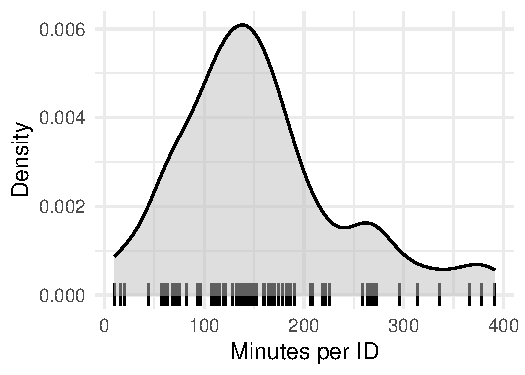
\includegraphics{Quantex_interaction_paper_files/figure-latex/quantex-minutes-per-child-1} 

}

\caption{Video recording duration (in minutes) per Child in the Quantex Dataset.}\label{fig:quantex-minutes-per-child}
\end{figure}

\subsection{Annotation Strategy}\label{annotation-strategy}

The dataset annotations cover four key elements: persons, faces, gaze direction, and objects. Each detected person (or reflection) and face includes attributes like a unique ID, age, and gender. Gaze annotations indicate whether a person is looking at the child. Faces are annotated even if occluded or blurry, as long as key features remain visible.

The egocentric chest-mounted camera introduced challenges like motion blur and oblique angles, making gaze classification difficult, even for human annotators. Many frames had occluded or distorted gaze information. Objects are annotated only when actively interacted with and categorized into seven groups: book, screen, animal, food, toy, kitchenware, and other. The annotation strategy is summarized in Figure \ref{fig:camera-cvat-activity-classes}.

The Quantex dataset includes 634 videos, with 80 annotated, totaling 113799 frames. Every 30th frame (one per second) was annotated to balance workload while ensuring meaningful data. These annotations serve as ground truth for training a model to analyze the remaining videos. While video data underwent structured annotation and validation, audio data was analyzed in raw form.

\begin{figure}

{\centering 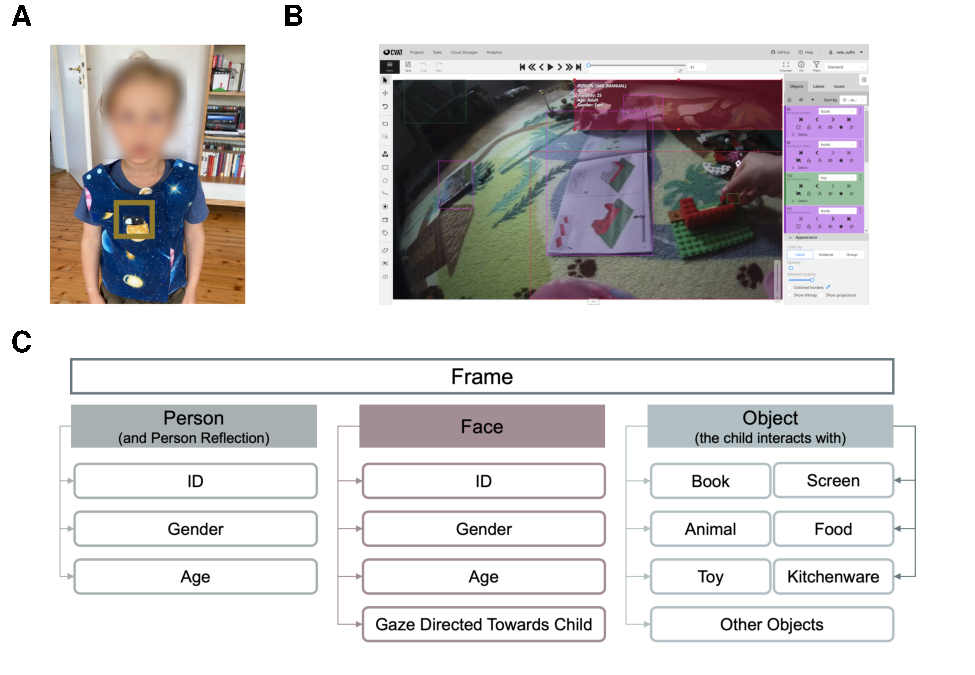
\includegraphics{Quantex_interaction_paper_files/figure-latex/camera-cvat-activity-classes-1} 

}

\caption{\textbf{A} – Vest with the embedded camera worn by the children, \textbf{B} – CVAT platform utilized for video annotation, \textbf{C} – Annotation Strategy in the Quantex dataset.}\label{fig:camera-cvat-activity-classes}
\end{figure}

\section{Automated Analysis Pipeline}\label{automatic-analysis}

Our automated analysis pipeline consists of four key modules: detection of person, faces, and objects, gaze classification, proximity heuristic, voice type classification. Each module operates independently, utilizing separate machine learning models. Except for the voice type classifier, all models were trained on the Quantex dataset.

The pipeline follows a sequential process:

\begin{itemize}
\tightlist
\item
  YOLO11x detection model identifies the presence of individuals (persons and faces) and types of objects the key child interacts with, both in social and independent play contexts, in the video frames.
\item
  Gaze classification determines whether detected faces are looking at the child.
\item
  Proximity heuristic estimates the distance between the child and others based on face size and aspect ratio.
\item
  Voice type classification detects the presence of speech and identifies whether the speaker is the key child, another child, or an adult.
\end{itemize}

By integrating these modules, our pipeline enables a comprehensive analysis of children's everyday experiences, capturing both social interactions and independent play.

In the following sections, we describe each module in detail, including training data, model architecture, and evaluation metrics. A full technical analysis of each algorithm is provided in the \hyperref[supplementary-material]{Supplementary Material}.

\subsection{Yolo11x: Multi-Class Detection of Persons, Faces, and Objects}\label{yolo11x}

We used Ultralytics' YOLO11, a ``state-of-the-art real-time object detector'' (Jocher \& Qiu, 2024), pretrained on COCO (Lin et al., 2014). Released in October 2024, YOLO11 introduces C2PSA and C3K2 blocks for enhanced spatial attention and feature aggregation (Khanam \& Hussain, 2024). Given our egocentric dataset's dynamic nature, we selected YOLO11x, the largest model (56.9M parameters, 194.9 GFLOPs), offering the highest accuracy (mAP\(^{val}_{50-95}\) = 54.7) among YOLO11 variants.

\subsubsection{Dataset Annotation and Preprocessing}\label{dataset-annotation-and-preprocessing}

Egocentric recordings often include the child's body parts, so we assigned all individuals the label ``person'' with unique IDs, marking the key child as ID = 1. This ID was later mapped to a ``child body parts'' category. We refined the ``person'' and ``face'' labels by:

\begin{itemize}
\tightlist
\item
  Differentiating the key child from others.
\item
  Distinguishing adults from children/infants in both full-body and face detections.
\end{itemize}

Our fine-tuned YOLO11x model also classifies five key object categories: toy, book, kitchenware, screen, and other object. Due to low occurrences, ``animal'' and ``food'' were merged into ``other object,'' ensuring all final object classes had at least 2,000 instances.

The Quantex dataset contains 634 videos recorded at 30fps, resulting in 19023571 frames. We annotated 80 videos (113799 frames) and applied a stratified 80/10/10 split to preserve class distributions across training (91039), validation (11380), and testing (11380) sets.

\subsubsection{Training and Evaluation}\label{training-face}

We trained YOLO11x on a Linux server (Quadro RTX 8000 GPU, 48-core Intel Xeon CPU, 188 GB RAM) for 86 epochs (200 hours) using 640px images, a batch size of 16, cosine annealing learning rate scheduling (Loshchilov \& Hutter, 2017), and early stopping after 10 epochs without improvement(max 200).

The loss function comprises Box Loss, Classification Loss, and Distribution Focal Loss (DFL) (Li et al., 2020; Terven, Cordova-Esparza, Ramirez-Pedraza, Chavez-Urbiola, \& Romero-Gonzalez, 2024), ensuring precise localization and classification. Evaluation with a confusion matrix and precision-recall curves showed strong class separation, achieving a precision of 0.91, recall of 0.80, F1-score of 0.85, and mAP of 0.87 (Table \ref{tab:det-metrics-short}).

\begin{table}[tbp]

\begin{center}
\begin{threeparttable}

\caption{\label{tab:det-metrics-short}YOLO11x detection metrics on the Quantex dataset, reporting mAP@0.5, precision, recall, and F1-score across all classes.}

\begin{tabular}{llll}
\toprule
mAP@0.5 & \multicolumn{1}{c}{Precision} & \multicolumn{1}{c}{Recall} & \multicolumn{1}{c}{F1-Score}\\
\midrule
0.870 & 0.91 & 0.80 & 0.85\\
\bottomrule
\end{tabular}

\end{threeparttable}
\end{center}

\end{table}

\begin{figure}

{\centering \includegraphics{Quantex_interaction_paper_files/figure-latex/det-detection-examples-short-1} 

}

\caption{Detection examples for the YOLO11x detection model trained on the Quantex dataset.}\label{fig:det-detection-examples-short}
\end{figure}

While people, books, and screens had high AP scores, ``toy'' (0.77), ``kitchenware'' (0.77), and ``other object'' (0.82) were often misclassified as background, likely due to selective annotation of child-interacted objects. Similarly, ``infant/child'' and ``infant/child face'' had false negatives, possibly due to occlusions and limited annotated samples. Future improvements could address these issues by expanding annotations and applying data augmentation. Overall, the model effectively detects people, faces, and key objects, as illustrated in Figure \ref{fig:det-detection-examples-short}.

\subsection{Yolo11x-cls: Gaze Classification}\label{yolo11x-cls}

Selecting a gaze classification model for our egocentric dataset presented challenges due to blurry, partially occluded faces captured at varying angles. Many gaze estimation methods rely on high-quality eye images (Zhang, Sugano, Fritz, \& Bulling, 2015, 2016), making them unsuitable for our data. Additionally, rather than predicting fine-grained gaze direction (e.g., left or right), our focus is on the binary classification of whether a person's gaze is directed toward the child or not.

Given these constraints, we implemented ResNet- and YOLO-based models, selecting Ultralytics' YOLO11x (Jocher \& Qiu, 2024) after preliminary testing. YOLO11x-cls, the largest variant with 28.4M parameters, achieved the highest accuracy (acc\_top1 = 79.5) on our dataset. Its architectural enhancements, such as the C2PSA block, improve attention to critical regions, ensuring robust gaze detection under real-world conditions.

\subsubsection{Data Annotation and Preprocessing}\label{data-annotation-and-preprocessing}

We defined gaze as directed towarda the child if a person's gaze was oriented toward the child's face, body, or general direction. Each detected face was labeled as ``gaze'' or ``no gaze.''

For training, we extracted cut-out faces from 64 videos, resulting in 20889 frames. Since only 21.25\% of faces were labeled ``gaze,'' we applied stratified splitting and data augmentation to balance the training set while keeping validation and testing sets in their natural distribution (Table \ref{tab:gaze-dataset-splits-short}).

\subsubsection{Training and Evaluation}\label{training-and-evaluation}

We trained YOLO11x-cls for 37 epochs on a Linux server, using an image size of 640, batch size of 16, cosine annealing (Loshchilov \& Hutter, 2017), and early stopping after 10 epochs. Training took 10.40 hours.

The model achieved a precision of 0.64, a recall of 0.77 recall, and an F1-score of 0.70 (Table \ref{tab:gaze-metrics-short}). The cross-entropy loss curves for training and validation steadily decreased, with no signs of overfitting, indicating good generalization (see \hyperref[sup-yolo11x-cls]{Gaze Classification} in the Supplementary Material for details).

\begin{table}[tbp]

\begin{center}
\begin{threeparttable}

\caption{\label{tab:gaze-dataset-splits-short}Dataset splits for the YOLO11x gaze classification model trained on the Quantex dataset. The table shows the total number of frames, as well as the number of frames with gaze and no gaze in the training, validation, and testing datasets after data augmentation of the minority class (Gaze). 'Gaze' indicates frames where the person's gaze is directed towards the child, while 'No Gaze' indicates frames where the person's gaze is not directed towards the child. Ratios are given in percentages.}

\begin{tabular}{lllllll}
\toprule
Quantex & \multicolumn{1}{c}{Train Ratio (\%)} & \multicolumn{1}{c}{Training} & \multicolumn{1}{c}{Val \& Test Ratio (\%)} & \multicolumn{1}{c}{Validation} & \multicolumn{1}{c}{Testing} & \multicolumn{1}{c}{Total}\\
\midrule
Gaze & 50 & 13160 & 79 & 1645 & 1646 & 16451\\
No Gaze & 50 & 13160 & 21 & 443 & 445 & 14048\\
Total & 100 & 26320 & 100 & 2088 & 2091 & 30499\\
\bottomrule
\end{tabular}

\end{threeparttable}
\end{center}

\end{table}

Despite strong performance, the egocentric perspective introduces challenges. Faces are often occluded or blurred, making gaze classification difficult---even for human annotators, who occasionally required a second inspection. Cut-off faces lacking visible eyes pose an additional issue, requiring the model to rely on head orientation and other facial features, which sometimes leads to misclassification.

Future work could incorporate temporal cues or additional facial landmarks to improve performance. However, given our dataset constraints, YOLO11x-cls provides a solid foundation for analyzing gaze in egocentric video data.

\begin{table}[tbp]

\begin{center}
\begin{threeparttable}

\caption{\label{tab:gaze-metrics-short}Evaluation metrics for the YOLO11x-cls gaze classification model, for detecting if a person is looking at the key child.}

\begin{tabular}{lll}
\toprule
Precision & \multicolumn{1}{c}{Recall} & \multicolumn{1}{c}{F1-Score}\\
\midrule
0.64 & 0.77 & 0.70\\
\bottomrule
\end{tabular}

\end{threeparttable}
\end{center}

\end{table}

\subsection{Proximity Heuristic}\label{proximity-heuristic}

Proximity plays a key role in social interaction, offering insights into the nature of relationships and social engagement (Hernández-Heredia, Reyes-Manzano, Flores-Hernández, Ramos-Fernández, \& Guzmán-Vargas, 2024; Janssen et al., 2024; Onnela et al., 2014). As our dataset lacks explicit proximity labels, we developed a heuristic method to estimate the distance between the child and others.

\subsubsection{Formula for Proximity Estimation}\label{formula-for-proximity-estimation}

We estimate proximity using the size of detected face bounding boxes, assuming that larger boxes indicate closer individuals and smaller ones suggest greater distance. The proximity value is calculated based on face area (width × height) and compared to reference sizes: one for a face within arm's reach and another for a more distant face (e.g., in the background or outdoors).

Since face area decreases quadratically as distance increases, a simple linear mapping would exaggerate differences for close faces and minimize them for distant ones. To address this, we apply logarithmic scaling, ensuring a more accurate proximity score between 0 and 1:

\[
\text{Proximity} = \frac{\ln(\text{Face Area}) - \ln(\text{Max Reference Area})}{\ln(\text{Min Reference Area}) - \ln(\text{Max Reference Area})}
\]

Where:

\begin{itemize}
\tightlist
\item
  \(\textbf{Face Area}\): Width × height of the detected face's bounding box.
\item
  \(\textbf{Max Reference Area}\): Area of the furthest detectable face.
\item
  \(\textbf{Min Reference Area}\): Area of the closest detectable face.
\end{itemize}

This logarithmic transformation compresses proximity values for large faces (close to the camera) and stretches them for small faces (farther away), aligning with human perceptual sensitivity to relative size changes (Stevens \& Marks, 2017).

\begin{figure}

{\centering \includegraphics{Quantex_interaction_paper_files/figure-latex/proximity-classifications-1} 

}

\caption{Proximity Heuristic Examples. Example \textbf{A} shows a face far away from the camera (proximity score = 0.07), example \textbf{B} depicts a face slighlty closer (proximity score = 0.2). Example \textbf{C} shows a face quite close to the camera (proximity score = 0.6), and example \textbf{D} illustrates a face extremely close to the camera (proximity score = 1).}\label{fig:proximity-classifications}
\end{figure}

\subsubsection{Incorporating Width-to-Height Ratio}\label{incorporating-width-to-height-ratio}

Additional to face size, we use the faces' width-to-height ratio as cues for proximity.
Based on reference images of full, front-facing faces, we define an expected aspect ratio for adults and children. If a detected face's ratio deviates significantly, we infer that the face is extremely close to the camera, causing partial cropping of the bounding box. If the deviation exceeds a defined threshold (\(\epsilon\)), the proximity score is set to 1.

This heuristic approach, which combines face area and aspect ratio, provides an efficient and interpretable method for estimating proximity without requiring additional sensors or depth information. Its validity is supported by a strong Pearson correlation coefficient (r = 0.95) between the heuristic estimates and human-annotated proximity values, based on 364 annotated frames from the Quantex dataset. This high correlation indicates that the heuristic effectively captures the relative distances between the child and others in the recordings, thereby enabling the integration of spatial dynamics into our interaction analyses. Examples of proximity estimations are shown in Figure @ref((fig:proximity-classifications), illustrating the range of proximity scores from 0 (far away) to 1 (extremely close).

\subsection{Participation Role Classification (PRC)}\label{voice-type}

Regarding the audio component of our interaction analysis, we classified audio by speaker and intended target into four types: key child (KCHI), child-directed speech (CDS), overheard speech (OHS), and general speech (SPEECH). To achieve this, we adapted the open-source Voice Type Classifier (VTC) (Lavechin, Bousbib, Bredin, Dupoux, \& Cristia, 2020), designed to distinguish key child, other child, female adult, male adult, and general speech. The resulting architecture, referred to as the Participation Role Classifier (PRC), uses a SincNet front-end, a 3-layer bi-directional GRU (512 units), and extended input segments (4.0s) to better model interaction patterns. On our labeled ChildLens dataset (CHILDLENS PAPER REFERENCE), the PRC achieved an average F1 score of 65.40, matching the original VTC's performance (57.30) and confirming its suitability for our data.

\section{Results}\label{results}

\subsection{Developmental Trends in Social Interaction}\label{developmental-trends-in-social-interaction}

\subsubsection{Age-related changes in social engagement}\label{age-related-changes-in-social-engagement}

\subsubsection{Gaze Direction Dynamics}\label{gaze-direction-dynamics}

\begin{itemize}
\tightlist
\item
  another interesting interaction aspect is the percentage of faces with gaze directed at the child and how this percentage develops over time. we furthermore analyse the percentage of adult faces with gaze directed at the child and the percentage of child faces with gaze directed at the child and whether there are differences between the age groups. as visible in Figure \ref{fig:gaze-patterns-by-age}, the percentage of faces with gaze directed at the child increases with age, with 3-year-olds showing the lowest percentage and 5-year-olds the highest. this trend is consistent for both adult and child faces, indicating a developmental shift towards more focused attention on the child.
\item
  overall the percentage of faces with gaze directed at the child do not show any age-related differences, neither for adult faces nor for child faces. in both face categories the percentage stay rather stable, as shown in Table \ref{tab:gaze-percentage-overall-comparison}. however, when comparing the percentage of adult and child faces with gaze directed at the child (child 64.55\% vs.~adult 70.80\%), we find that child faces are more likely to look at the child than adult faces, with a significant difference across all age groups. this suggests that children are more often the focus of attention in social interactions, regardless of the age of the interacting partner. while it often can also be possible that adults are present but do not interact with the child, the higher percentage of child faces with gaze directed at the child indicates that children are actively engaged in social interactions with the key child.
\end{itemize}

Another interesting interaction aspect is the percentage of faces with gaze directed at the child and how this percentage develops with increasing age of the key child. We furthermore analyze the percentage of adult faces with gaze directed at the child and the percentage of child faces with gaze directed at the child, and whether there are differences between the age groups. As visible in Figure \ref{fig:gaze-patterns}, the percentage of faces with gaze directed at the child stays rather stable across all age groups. This trend is consistent for both adult and child faces.

Overall, the percentage of faces with gaze directed at the child does not show any age-related differences, neither for adult faces nor for child faces. In both face categories, the percentages remain rather stable, as shown in Table (\textbf{ref?})(tab:gaze-percentage-overall-comparison). However, when comparing the percentage of adult and child faces with gaze directed at the child (child r adult\_gaze\_overall\% vs.~adult r child\_gaze\_overall\%), we find that child faces are more likely to look at the child than adult faces, with a significant difference across all age groups. This suggests that children are more often the focus of attention in social interactions, regardless of the age of the interacting partner. While it is often possible that adults are present but do not interact with the child, the higher percentage of child faces with gaze directed at the child indicates that children are actively engaged in social interactions with the key child.

\begin{figure}

{\centering 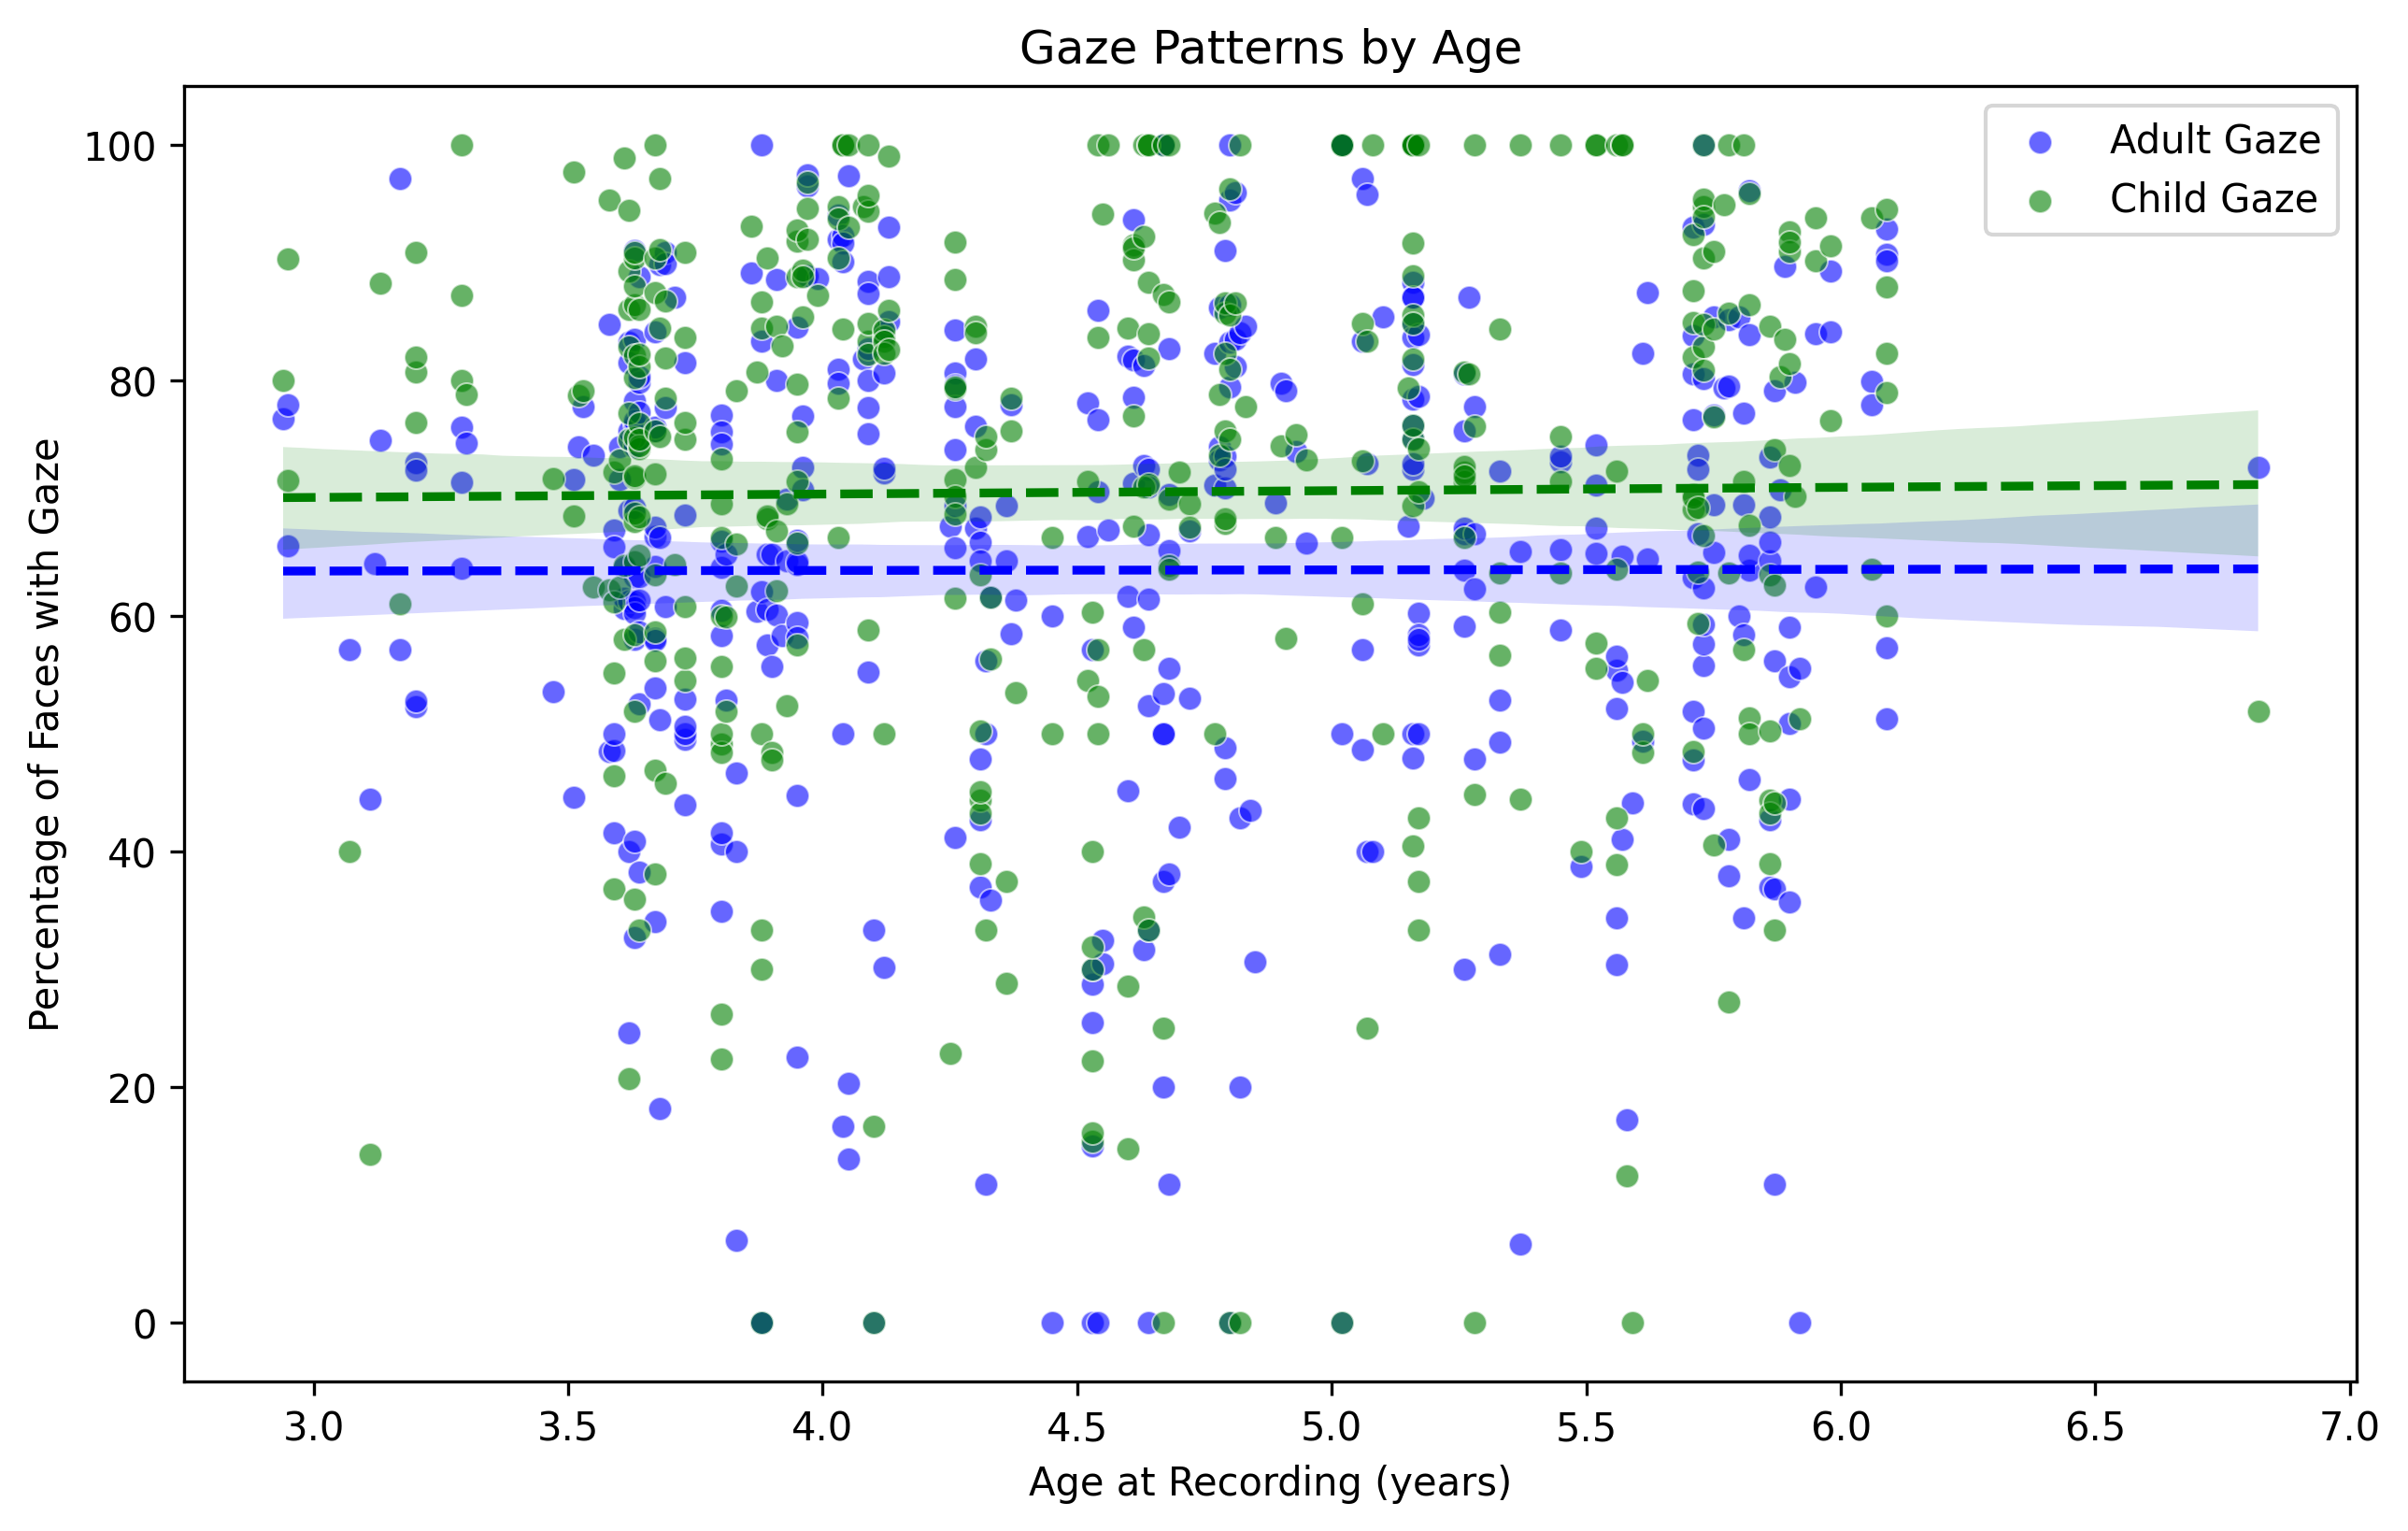
\includegraphics[width=450px]{images/gaze_patterns_by_age} 

}

\caption{Percentage of faces wth gaze directed at child across different age groups.}\label{fig:gaze-patterns}
\end{figure}

\begin{table}[tbp]

\begin{center}
\begin{threeparttable}

\caption{\label{tab:gaze-percentage-overall-comparison}Overall Adult vs. Child Gaze Comparison. The table shows the percentage of adult and child faces with gaze directed at the child across different age groups. The t-statistic and p-value are reported for the overall comparison and each age group comparison.}

\begin{tabular}{llllll}
\toprule
Group & \multicolumn{1}{c}{Adult Gaze (\%)} & \multicolumn{1}{c}{Child Gaze (\%)} & \multicolumn{1}{c}{t-stat} & \multicolumn{1}{c}{p-value} & \multicolumn{1}{c}{N}\\
\midrule
Overall & 64.55 & 70.80 & -5.191 & 0.0000*** & 401\\
Age 3 & 63.95 & 70.88 & -4.416 & 0.0000*** & 139\\
Age 4 & 64.90 & 69.74 & -1.924 & 0.0566 & 125\\
Age 5 & 64.85 & 71.68 & -3.172 & 0.0019** & 137\\
\bottomrule
\end{tabular}

\end{threeparttable}
\end{center}

\end{table}

\subsubsection{Presence of a Face}\label{presence-of-a-face}

\subsubsection{Presence of Gaze}\label{presence-of-gaze}

\subsubsection{Presence of Language}\label{presence-of-language}

\subsection{Co-occurrence of Aspects of Social Interaction}\label{co-occurrence-of-aspects-of-social-interaction}

\section{General Discussion}\label{general-discussion}

\newpage

\section{References}\label{references}

\newpage

\section{Supplementary Material}\label{supplementary-material}

\subsection{Outline}\label{outline}

This document contains supplementary material for the paper ``Exploring Aspects of Social Interaction in Children's Everyday Lives using Machine Learning: A Multimodal Analysis of the Quantex Dataset''. First, we provide an overview of the \hyperref[sup-participants]{Participant Recruitment and Data Collection}, including a detailed description of the \hyperref[sup-recruitment]{Recruitment and Data Collection} process. We then describe the \hyperref[sup-materials]{Materials} used in the study, followed by a structured overview of the \hyperref[sup-dataset]{Dataset}, including the \hyperref[sup-annotation-strategy]{Annotation Strategy}. Next, we outline the \hyperref[sup-automatic-analysis]{Automated Analysis Pipeline}, including \hyperref[sup-yolo11x]{YOLO11x: Multi-Class Detection of Persons, Faces, and Objects}, \hyperref[sup-yolo11x-cls]{YOLO11x-cls: Gaze Classification}), as well as \hyperref[sup-voice-type]{Voice Type Classification}. Finally, we report the \hyperref[sup-results]{Results} of the automated pipeline, evaluating the performance of the models when applied to all videos in the Quantex dataset.

\section{Methodology}\label{sup-methodology}

The following sections provide a detailed description of the data collection process, the structure and characteristics of the dataset, the annotation strategy, and the preprocessing applied to the data prior to analysis. Additionally, an overview of the automated analysis pipeline is provided, giving details about the models used for person and face detection, gaze classification, object detection, and the application of a pre-trained voice type classifier.

\subsection{Participants Recruitment and Data Collection}\label{sup-participants}

This study collected egocentric video recordings from 76 children, aged 3 to 5 years, over a span of 73 months {[}MB: in addition, it would be interesting to know in what time intervall the videos were collected for each child, also a more detailed overview of the number of children per age group would be nice{]}.

\subsubsection{Recruitment Process}\label{recruitment-process-1}

Participants were recruited from a mid-sized German city through an existing lab database, with approximately equal distribution across age groups (30\% 3-year-olds, 35\% 4-year-olds, 35\% 5-year-olds). The data collection process was approved by the local ethics committee, and all participating families provided written informed consent, allowing the researchers to use the data for scientific purposes. Participants were recruited from an internal lab database and contacted via phone. Parents received a detailed explanation of the study's purpose and procedures, consistent with the information in the study brochure. Families who agreed to participate were provided with a vest equipped with an embedded camera, which children were asked to wear for approximately two hours, with flexible extension options. For privacy protection, recordings were limited to the home environment. Recorded videos were securely stored on the MPI-EVA server and subsequently made available to parents. To enhance convenience, parents could choose to have the camera delivered to their home or workplace, or opt for self-pickup.

\subsubsection{Distribution of Study Materials and Instructions}\label{distribution-of-study-materials-and-instructions-1}

At the handover appointment, parents received one or two vests (multiple sizes available), a fully charged camera unit and comprehensive information on the study's purpose and data protection protocols. Parents received hands-on training on camera operation and were encouraged to practice using the equipment. The consent form required listing the participating child and documenting all individuals potentially captured in the recordings. Five copies of data privacy information sheets were provided for distribution to anyone who might be recorded. A follow-up call was scheduled to ensure recording success, typically planned for the weekend following the handover to ensure enough time for recoding.

\subsubsection{Return of Equipment and Final Data Confirmation}\label{return-of-equipment-and-final-data-confirmation-1}

On the scheduled date, parents were contacted to confirm recording success and assess any need for additional time. Flexible rescheduling was offered as needed. Once the recording was completed, a pickup or drop-off appointment was arranged to collect the completed consent form, vest, and camera. Parents were also asked to confirm their current email address for sharing the recordings. Children received a ``Labyrinth'' game as a thank for their participation.

\subsection{Materials}\label{sup-materials}

To capture children's everyday experiences, a wearable vest equipped with a \emph{PatrolEyes WiFi HD Infrared Police Body Camera} was used (Figure \ref{fig:camera-cvat-activity-classes}). The camera recorded high-definition video (1920x1080p at 30 fps) with a 140-degree wide-angle lens and also captured audio. Children were free to move around and engage in their usual activities at home without any interference or instructions given to their parents.

\subsection{Dataset Overview}\label{sup-dataset}

The Quantex dataset includes video and audio recordings from 76 children aged 3 to 5 years (M=4.53, SD=0.81). The dataset contains 167 videos from three-year-olds, 180 videos from four-year-olds, and 156 videos from five-year-olds. The number of videos per child varies, as parents decide when and how often to record. The recording duration per child ranges from 10.43 to 391.18 minutes (M=155.68, SD=82.62). The total duration of all video recordings in the dataset is 197.20 hours. Figure \ref{fig:sup-quantex-minutes-per-child} shows the distribution of video duration per child.

\begin{figure}

{\centering 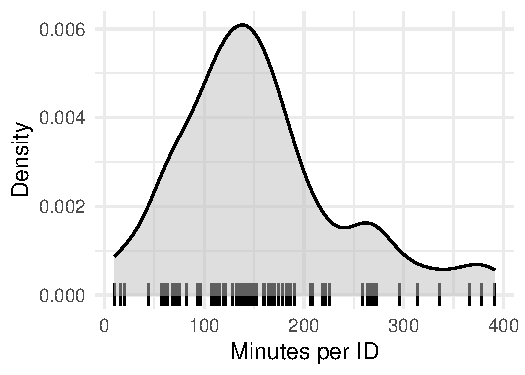
\includegraphics{Quantex_interaction_paper_files/figure-latex/sup-quantex-minutes-per-child-1} 

}

\caption{Video recording duration (in minutes) per Child in the Quantex Dataset.}\label{fig:sup-quantex-minutes-per-child}
\end{figure}

\subsection{Annotation Strategy}\label{sup-annotation-strategy}

The dataset annotations cover four key elements: persons, faces, gaze direction, and objects the child interacts with. For each detected person (or reflection of a person, such as in a mirror) and face, additional attributes are recorded, including a unique identifier, age (infant, child, teen, adult, unknown), and gender (female, male, unknown). Gaze information indicates whether a detected person's gaze is directed toward the child or not. Faces are annotated even when occluded or blurry to ensure comprehensive coverage of interactions. Partially visible faces are also annotated if key facial features, such as the nose, eyes, or mouth, remain identifiable.

The egocentric nature of our video data, recorded from a chest-mounted camera, posed additional challenges such as motion blur and oblique viewing angles, which made gaze classification difficult, even for human annotators. These factors contributed to occlusion or distortion of gaze information in many frames, making accurate gaze direction annotation particularly challenging.

Objects are annotated only when the child is actively interacting with them, either by holding them in their own hands or when another person in the interaction is holding the object in their hands. These objects are categorized into six distinct groups: book, screen, animal, food, toy, and kitchenware, with an additional category for other objects. The annotation strategy is summarized in Figure \ref{fig:sup-camera-cvat-activity-classes}.

The Quantex dataset consists of a total of 634 videos. However, only a subset of 80 videos was annotated, totaling 113799 frames. To balance workload while still obtaining meaningful annotations, we applied a frame sampling strategy, annotating every 30th frame, which corresponds to one frame per second. The goal of these annotations was to create ground truth data for training a model that can later be used to analyze the remaining videos in the dataset. While the video data was subject to structured annotation and validation, the audio data was used in its raw form without preprocessing for analysis.

\begin{figure}

{\centering 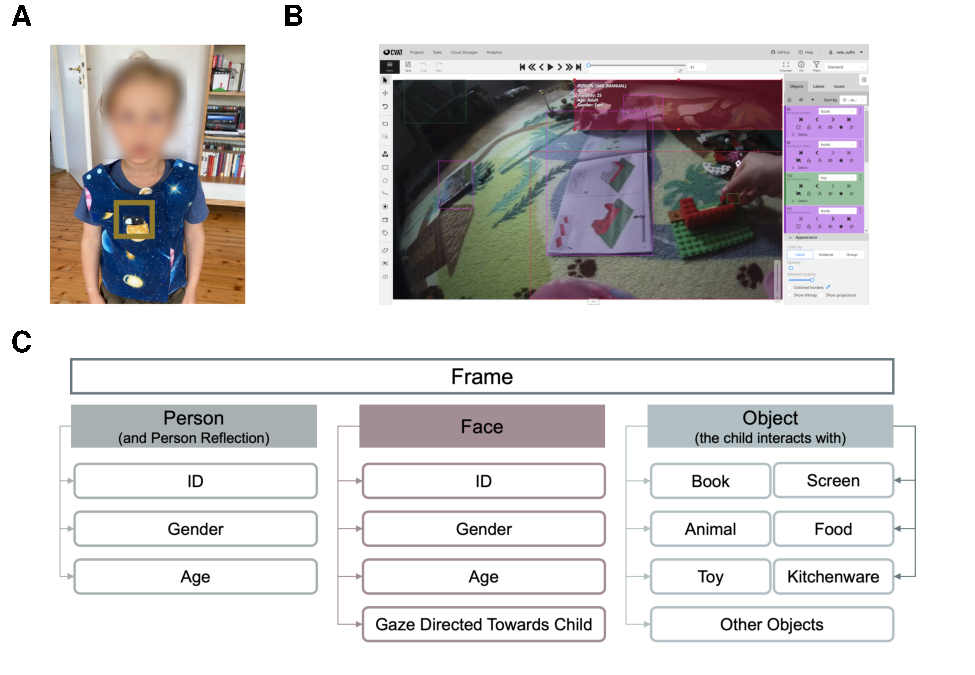
\includegraphics{Quantex_interaction_paper_files/figure-latex/sup-camera-cvat-activity-classes-1} 

}

\caption{\textbf{A} – Vest with the embedded camera worn by the children, \textbf{B} – CVAT platform utilized for video annotation, \textbf{C} – Annotation Strategy in the Quantex dataset.}\label{fig:sup-camera-cvat-activity-classes}
\end{figure}

\section{Automated Analysis Pipeline}\label{sup-automatic-analysis}

Our automated analysis pipeline consists of four key modules: person and face detection, gaze classification, object detection, and voice type classification. Each module operates independently, utilizing separate machine learning models. Except for the voice type classifier, all models were trained on the Quantex dataset.

The pipeline follows a sequential process:

\begin{verbatim}
1.  YOLO11x detection model identifies the presence of individuals (persons and faces) and types of objects the key child interacts with, both in social and independent play contexts, in the video frames.
2.  Gaze classification determines whether detected faces are looking at the child.
3.  Voice type classification detects the presence of speech and identifies whether the speaker is the key child, another child, or an adult.
\end{verbatim}

By integrating these modules, our pipeline enables a comprehensive analysis of children's everyday experiences, capturing both social interactions and independent play.

\subsection{YOLO11x: Multi-Class Detection of Persons, Faces, and Objects}\label{sup-yolo11x}

In our study, we utilized Ultralytics' YOLO11, the ``latest iteration in the Ultralytics YOLO series of real-time object detectors'' (Jocher \& Qiu, 2024), trained on the COCO dataset (Lin et al., 2014), a large-scale dataset containing labeled images for 80 object categories commonly found in everyday environments. COCO is widely used for object detection, instance segmentation, and keypoint detection tasks.

Released in October 2024, YOLO11 introduces architectural improvements such as the C2PSA block (Convolutional Block with Parallel Spatial Attention), which enhances spatial attention within feature maps, allowing the model to focus more precisely on critical areas of an image compared to previous YOLO versions. Additionally, YOLO11 incorporates the C3K2 block, designed to be faster and more efficient, enhancing the overall performance of the feature aggregation process (Khanam \& Hussain, 2024). These advancements make the YOLO11 detection model, pretrained on COCO, well-suited for training on our egocentric dataset, which captures dynamic movements from a camera perspective on chest height.

For our study, we utilized YOLO11x, the largest model in the YOLO11 model series, which has 56.9M parameters and 194.9 GFLOPs. With the highest accuracy (mAP\(^{val}_{50-95}\) = 54.7) among YOLO11 variants, YOLO11x, combined with its architectural advancements, was the optimal choice for our task, as we had the computational resources to support running a larger model.

\subsubsection{Dataset Annotation and Preprocessing}\label{dataset-annotation-and-preprocessing-1}

Our dataset presents unique challenges due to its egocentric viewpoint, as body parts of the child wearing the camera frequently appear in the footage. To prevent misclassification, we employ a dedicated annotation scheme where all individuals are labeled as ``person'' with unique IDs, consistently assigning the key child (child wearing the camera) ID = 1. During preprocessing, we map this ID to a separate ``child body parts'' category to distinguish the child's presence from other individuals.

Additionally, we refine the ``person'' and ``face'' categories beyond standard YOLO models by:

\begin{itemize}
\tightlist
\item
  Differentiating the key child from other individuals.
\item
  Distinguishing adults from children/infants in both full-body detections and faces.
\end{itemize}

Our fine-tuned YOLO11 model also classifies five object categories relevant to the child's interactions: toy, book, kitchenware, screen, and other object. Due to low occurrences, ``animal'' (19 instances, 0.015\%) and ``food'' (1,115 instances, 0.84\%) were included into ``other object'', leaving five final object categories with at least 2,000 instances each.

\subsubsection{Dataset Splitting}\label{dataset-splitting}

The full Quantex dataset consists of 634 videos, all recorded at 30fps, resulting in 19023571 frames. From this dataset, we annotated 80 videos, totaling 113799 frames. Prior to splitting this dataset into training, validation, and testing datasets, we analyzed how often each class was present in the dataset. The distribution, displayed in detail in Table \ref{tab:det-class-distribution}, revealed an imbalance, with the ``Adult'' class being the most frequent. To address this imbalance, we applied a stratified split to ensure that each dataset preserved the original class distribution. Following an 80/10/10 split, the final datasets consisted of 91039 frames for training (80\%), 11380 frames for validation (10\%), and 11380 frames for testing (10\%), ensuring an accurate evaluation of model performance relative to real-world data distribution (see Figure \ref{tab:det-dataset-splits}).

\begin{table}[tbp]

\begin{center}
\begin{threeparttable}

\caption{\label{tab:det-class-distribution}Dataset splits for the YOLO11 detection model trained on the Quantex dataset. The table shows the distribution of annotated persons, faces, and objects in the training, validation, and testing datasets.}

\begin{tabular}{lllll}
\toprule
Class & \multicolumn{1}{c}{Training} & \multicolumn{1}{c}{Validation} & \multicolumn{1}{c}{Testing} & \multicolumn{1}{c}{Total}\\
\midrule
Adult & 25706 & 3213 & 3213 & 32132\\
Child/Infant & 22403 & 2801 & 2800 & 28004\\
Adult Face & 8669 & 1083 & 1084 & 10836\\
Child/Infant Face & 6756 & 844 & 845 & 8445\\
Book & 8370 & 1046 & 1046 & 10462\\
Toy & 13870 & 1734 & 1733 & 17337\\
Kitchenware & 1915 & 239 & 240 & 2394\\
Screen & 3374 & 422 & 422 & 4218\\
Other Object & 15608 & 1950 & 1950 & 19508\\
\bottomrule
\end{tabular}

\end{threeparttable}
\end{center}

\end{table}

\begin{table}[tbp]

\begin{center}
\begin{threeparttable}

\caption{\label{tab:det-dataset-splits}Number of frames in the training, validation, and testing datasets for the YOLO11 detection model.}

\begin{tabular}{lllll}
\toprule
 & \multicolumn{1}{c}{Training} & \multicolumn{1}{c}{Validation} & \multicolumn{1}{c}{Testing} & \multicolumn{1}{c}{Total}\\
\midrule
Number of frames & 91039 & 11380 & 11380 & 113799\\
\bottomrule
\end{tabular}

\end{threeparttable}
\end{center}

\end{table}

\subsubsection{Training and Convergence}\label{sup-training-face}

Model training was conducted on a Linux server equipped with an Intel(R) Xeon(R) Silver 4214Y CPU @ 2.20GHz with 48 cores, a Quadro RTX 8000 GPU and 188 GB of RAM. The model was trained for a total of 86 epochs, taking 200 hours to complete. Training utilized YOLO11's built-in data augmentation, an image size of 640, a batch size of 16, a cosine annealing learning rate scheduler (Loshchilov \& Hutter, 2017), and early stopping after 10 epochs without improvement, with a maximum of 200 epochs.

\begin{figure}

{\centering 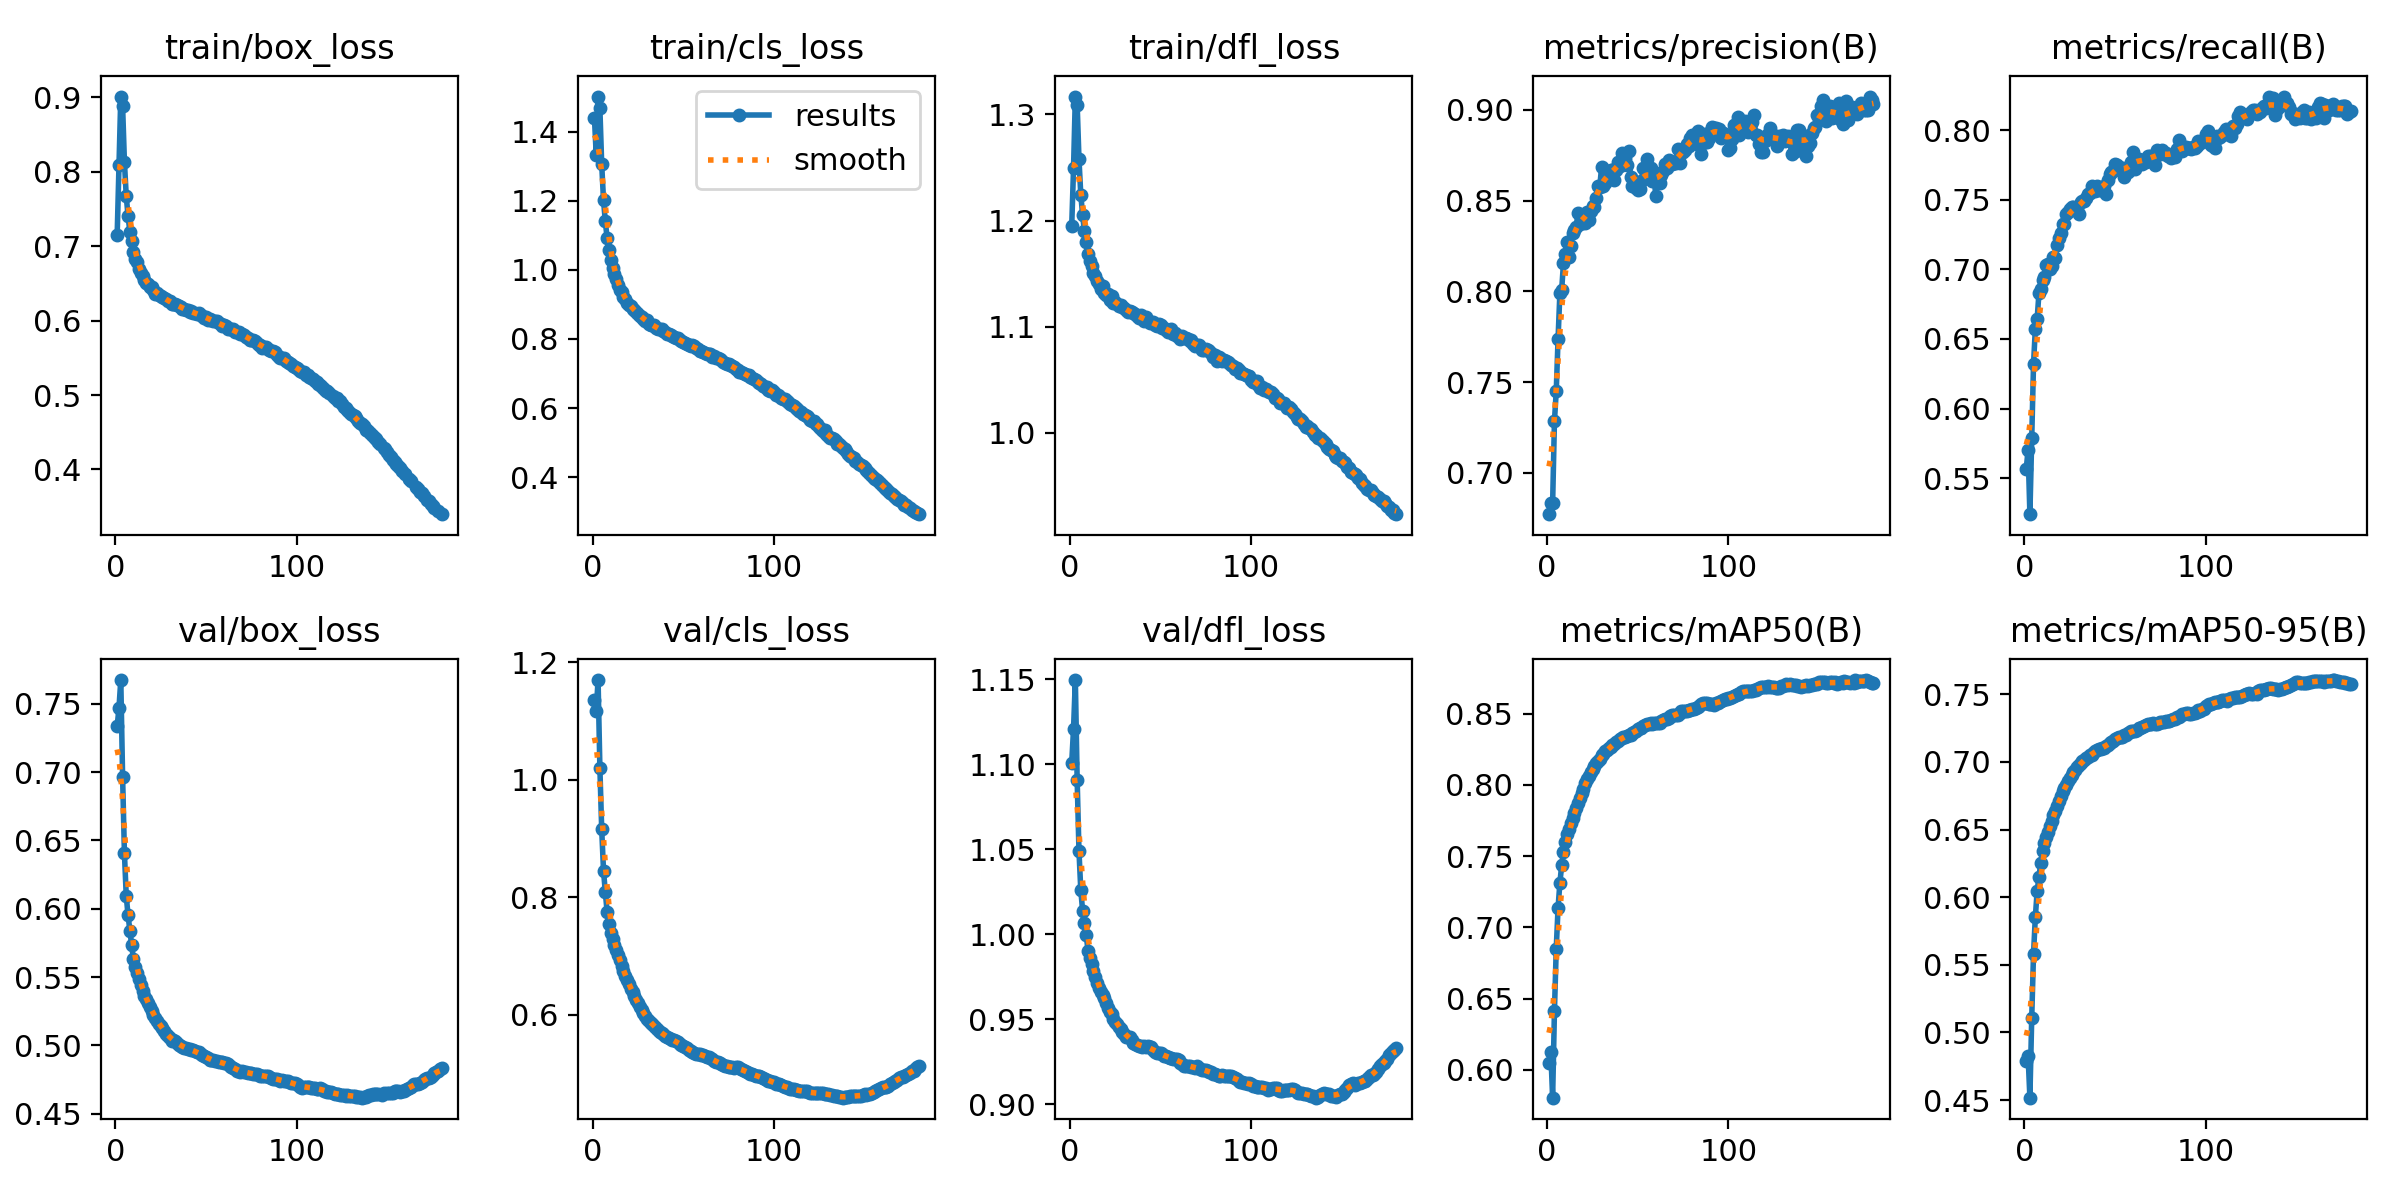
\includegraphics[width=450px]{images/yolo_loss_curves} 

}

\caption{Training and Validation Loss Curves for the YOLO11x detection model.}\label{fig:det-loss-curves}
\end{figure}

The loss function of the YOLO11 model comprises three main components: Box Loss, Classification Loss, and Distribution Focal Loss (DFL) (Li et al., 2020; Terven et al., 2024). \emph{Box Loss} quantifies the difference between predicted bounding boxes and ground truth boxes, ensuring precise localization of detected persons, faces and objects by penalizing inaccuracies in position and size. \emph{Classification Loss} (DFL) evaluates the model's ability to correctly assign detected instances to their respective classes, reducing false positives and false negatives. \emph{Distribution Focal Loss} enhances the model's ability to detect challenging persons, faces and objects, particularly small or partially occluded ones, by refining the localization of bounding box coordinates and emphasizing hard-to-detect instances. Together, these loss components contribute to a more robust and accurate detection model.

During the training process, we observed that all three loss components decreased over time, indicating effective learning and improved performance, as visible in in Figure \ref{fig:det-loss-curves}. A steady decrease in Box Loss indicates that the model is becoming increasingly accurate in localizing persons, faces and objects within frames. Similarly, the steady convergence of the Classification Loss reveals the model's increasing ability to reliably classifiy the detected instance in one of the relevant classes. The decrease in DFL over time indicates that the model is getting better at focusing on and correctly identifying difficult-to-detect persons, faces or objects, which improves its overall detection capabilities. Conclusively, the loss curves show that the model effectively learned to localize and identify the target classes during the training period.

\begin{table}[tbp]

\begin{center}
\begin{threeparttable}

\caption{\label{tab:det-map_all}Mean Average Precision (mAP@0.5) for the YOLO11x detection model trained on the Quantex dataset. The table shows the mAP@0.5 for each class.}

\begin{tabular}{ll}
\toprule
class & \multicolumn{1}{c}{mAP@0.5}\\
\midrule
infant/child & 0.87\\
adult & 0.95\\
infant/child face & 0.85\\
adult face & 0.95\\
child body parts & 0.97\\
book & 0.94\\
toy & 0.78\\
kitchenware & 0.81\\
screen & 0.96\\
other object & 0.83\\
\bottomrule
\end{tabular}

\end{threeparttable}
\end{center}

\end{table}

\begin{table}[tbp]

\begin{center}
\begin{threeparttable}

\caption{\label{tab:det-detection-metrics-detailed}Detection metrics for the YOLO11x detection model trained on the Quantex dataset. The table reports mean Average Precision at IoU 0.5 (mAP@0.5), along with the averaged precision, recall, and F1-score across all classes.}

\begin{tabular}{llll}
\toprule
mAP@0.5 & \multicolumn{1}{c}{Precision} & \multicolumn{1}{c}{Recall} & \multicolumn{1}{c}{F1-Score}\\
\midrule
0.870 & 0.91 & 0.80 & 0.85\\
\bottomrule
\end{tabular}

\end{threeparttable}
\end{center}

\end{table}

\begin{figure}

{\centering 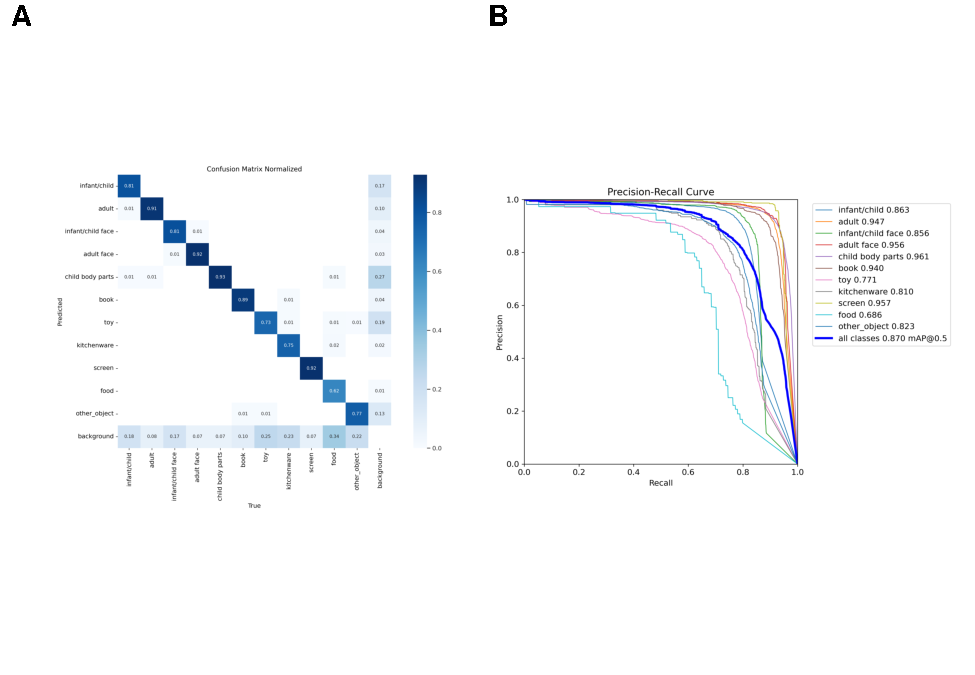
\includegraphics{Quantex_interaction_paper_files/figure-latex/det-metrics-1} 

}

\caption{\textbf{A} - Confusion Matrix for the YOLO11x detection model trained on the Quantex dataset. \textbf{B} - Precision-Recall Curve for the YOLO11x detection model.}\label{fig:det-metrics}
\end{figure}

\begin{figure}

{\centering \includegraphics{Quantex_interaction_paper_files/figure-latex/det-detection-examples-1} 

}

\caption{Detection examples for the YOLO11x detection model trained on the Quantex dataset.}\label{fig:det-detection-examples}
\end{figure}

\subsubsection{Model Evaluation Metrics}\label{model-evaluation-metrics}

The performance of the object detection model was evaluated using a confusion matrix and precision-recall (PR) curves. The YOLO11 model achieved a precision of 0.91 and a recall of 0.80 on the testing set, resulting in an F1-score of 0.85. The F1 metric is particularly important as it reflects both the accuracy of identifying each class instance (precision) and the model's ability to detect all occurrences of the class (recall). The normalized confusion matrix (see figure \ref{fig:det-metrics}) reveals strong overall performance with mean Average Precision across all classes mAP=0.87. The averaged precision-recall curve remains close to the top-left corner and signifies that the model maintains high precision and recall across various thresholds, underscoring its effectiveness in detecting the different classes.

To further refine detection results, we adjusted the built-in non-max suppression (NMS) threshold. YOLO already applies an NMS threshold of 0.7, where detections of the same class with an Intersection over Union (IoU) exceeding this threshold are suppressed. After evaluating different thresholds, we set the NMS IoU to 0.5, as this provided the best F1-score. However, this default NMS is only applied to bounding boxes of the same class, and manual inspection of detections revealed that some faces and persons were redundantly detected in multiple classes (e.g., a face detected as both ``adult face'' and ``child face'').

To address this issue, we implemented a custom cross-class NMS to remove duplicate detections across all classes. Using the same NMS logic, we applied an IoU threshold of 0.9 to ensure only nearly identical bounding boxes were removed while retaining valid detections. In cases where two overlapping bounding boxes exceeded this threshold, we kept the detection with the higher confidence score to minimize incorrect suppressions. This adjustment significantly reduced redundant detections while preserving true positive detections, leading to a more accurate and reliable final inference output.

Notably, the confusion matrix demonstrates minimal confusion between most classes, indicating that the model can effectively distinguish between them (see Figure \ref{fig:det-metrics}). A closer look at class-wise performance reveals that the model excels in detecting people and certain objects. The ``infant/child,'' ``adult,'' and ``adult face'' classes, as well as ``child body parts,'' ``infant/child face,'' ``book,'' and ``screen,'' all achieve high Average Precision (AP) scores. This indicates that the model reliably identifies these categories with strong precision and recall (see figure \ref{fig:det-metrics}).

On the other hand, some object classes remain more challenging. In particular, the ``toy,'' ``kitchenware,'' and ``other object'' categories exhibit lower AP scores of 0.77, 0.77, and 0.82, respectively. The confusion matrix confirms that 22\% of ``kitchenware'' and 22\% of ``toy'' instances are frequently misclassified as ``background.'' This issue likely stems from the annotation strategy, which prioritized labeling only objects that the child directly interacted with. As a result, other visually similar objects in the background remain unannotated, introducing ambiguity during training. Additionally, ``infant/child'' and ``infant/child face'' also show notable false negative rates of 17\%, further contributing to misclassification. These findings suggest that increasing the number of annotated samples---particularly for objects with which the child interacts with---could improve detection performance. Future work could also explore model refinements or data augmentation techniques to enhance the detection of small, occluded, or partially visible objects. In conclusion, the YOLO11 model demonstrates strong performance in detecting people, faces, and several object classes, as displayed in Figure \ref{fig:det-detection-examples}.

\subsection{YOLO11x-cls: Gaze Classification}\label{sup-yolo11x-cls}

Selecting an appropriate model for gaze classification in our automated pipeline presented unique challenges due to the egocentric perspective of our dataset. Many gaze estimation methods rely on high-quality eye images, either extracted separately (Zhang et al., 2015) or as part of the full face (Zhang et al., 2016). However, our dataset often contains blurry or partially occluded faces captured at varying angles, making such approaches not suitable. Additionally, rather than predicting fine-grained gaze direction (e.g., left or right), our focus is on the binary classification of whether a person's gaze is directed toward the child or not.

Cheng, Wang, Bao, and Lu (2021) provides an overview of the challenges and recent advancements in gaze estimation methods, including approaches that incorporate temporal information, such as Gaze360 (Kellnhofer, Recasens, Stent, Matusik, \& Torralba, 2019). While these methods improve tracking across frames, they are not the primary focus of our study, as we analyze social interactions on a frame-by-frame basis.

Given these constraints of our dataset, we opted for a CNN-based approach, which could be trained on ground truth annotations. Recent studies (Shah et al., 2022; Zhang et al., 2020; Zhang, Sugano, Fritz, \& Bulling, 2019) have explored different CNN based gaze estimation architectures, among which are VGG, ResNet or YOLO architectures. Based on these findings, we implemented a ResNet and YOLO-based model for binary classification (gaze directed toward the child or not). After conducting preliminary tests, Ultralytics' YOLO11 architecture (Jocher \& Qiu, 2024) demonstrated the best performance, which led us to select the YOLO11x classification model, pretrained on ImageNet, for our gaze classification task.

We fine-tuned YOLO11x-cls, the largest model in the YOLO11 classification series, which has 28.4M parameters. The model achieved the highest accuracy among all YOLO11 variants (acc\_top1 = 79.5), making it the optimal choice for gaze classification in our dataset. Moreover YOLO11's architectural enhancements, such as the C2PSA block, improve the model's ability to focus on critical regions within an image, ensuring robust detection of visual attention toward the child, even under challenging real-world conditions.

\subsubsection{Data Annotation and Preprocessing}\label{data-annotation-and-preprocessing-1}

We defined gaze as being ``directed toward the child'' when a person's gaze was oriented toward the child's face, body, or general direction of the child. This included instances where the person was looking directly at the camera (worn by the child) or slightly upwards, allowing for an estimation of the likely position of the child's head. Each detected face was annotated as either ``gaze'' (gaze directed at the child) or ``no gaze'' (gaze directed elsewhere).

\subsubsection{Dataset Splitting}\label{dataset-splitting-1}

For the gaze classification task, we utilized a subset of the Quantex dataset, focusing specifically on frames containing annotated faces. This subset consisted of cut-out faces extracted from the annotated face bounding boxes, resulting in 20889 frames from 64 annotated videos. An analysis of the gaze labels showed that 21.25\% of the faces were annotated as having gaze directed toward the child, leading to a class imbalance.

To maintain the original distribution of gaze labels across datasets, we first applied stratified dataset splitting, ensuring that the training, validation, and testing sets reflected the natural ratio of gaze and non-gaze frames. To address class imbalance in the training dataset, we applied data augmentation to increase the number of gaze frames. Since our dataset was already a subset of the Quantex dataset, downsampling to achieve balance would have resulted in a loss of valuable data. As a result, the final dataset included a balanced training set with 50\% gaze and 50\% no-gaze frames, while the validation and testing sets retained their original, unbalanced distribution. The final data distribution is presented in Table \ref{tab:gaze-dataset-splits}, with 26320 frames in the training set, 2088 frames in the validation set, and 2091 frames in the testing set.

\begin{table}[tbp]

\begin{center}
\begin{threeparttable}

\caption{\label{tab:gaze-dataset-splits}Dataset splits for the YOLO11x gaze classification model trained on the Quantex dataset. The table shows the total number of frames, as well as the number of frames with gaze and no gaze in the training, validation, and testing datasets after data augmentation of the minority class (Gaze). 'Gaze' indicates frames where the person's gaze is directed towards the child, while 'No Gaze' indicates frames where the person's gaze is not directed towards the child. Ratios are given in percentages.}

\begin{tabular}{lllllll}
\toprule
Quantex & \multicolumn{1}{c}{Train Ratio (\%)} & \multicolumn{1}{c}{Training} & \multicolumn{1}{c}{Val \& Test Ratio (\%)} & \multicolumn{1}{c}{Validation} & \multicolumn{1}{c}{Testing} & \multicolumn{1}{c}{Total}\\
\midrule
Gaze & 50 & 13160 & 79 & 1645 & 1646 & 16451\\
No Gaze & 50 & 13160 & 21 & 443 & 445 & 14048\\
Total & 100 & 26320 & 100 & 2088 & 2091 & 30499\\
\bottomrule
\end{tabular}

\end{threeparttable}
\end{center}

\end{table}

\subsubsection{Training and Convergence}\label{training-and-convergence}

We trained the gaze classification model on the same Linux server used for person and object detection model training. For details, see \hyperref[sup-training-face]{Training and Convergence}. Training ran for 37 epochs, completing in 10.40 hours . Similar to the YOLO detection model, we used an input image size of 640, a batch size of 16, a cosine annealing learning rate scheduler (Loshchilov \& Hutter, 2017), and early stopping after 10 epochs without improvement, with a maximum of 200 epochs.

\begin{figure}

{\centering 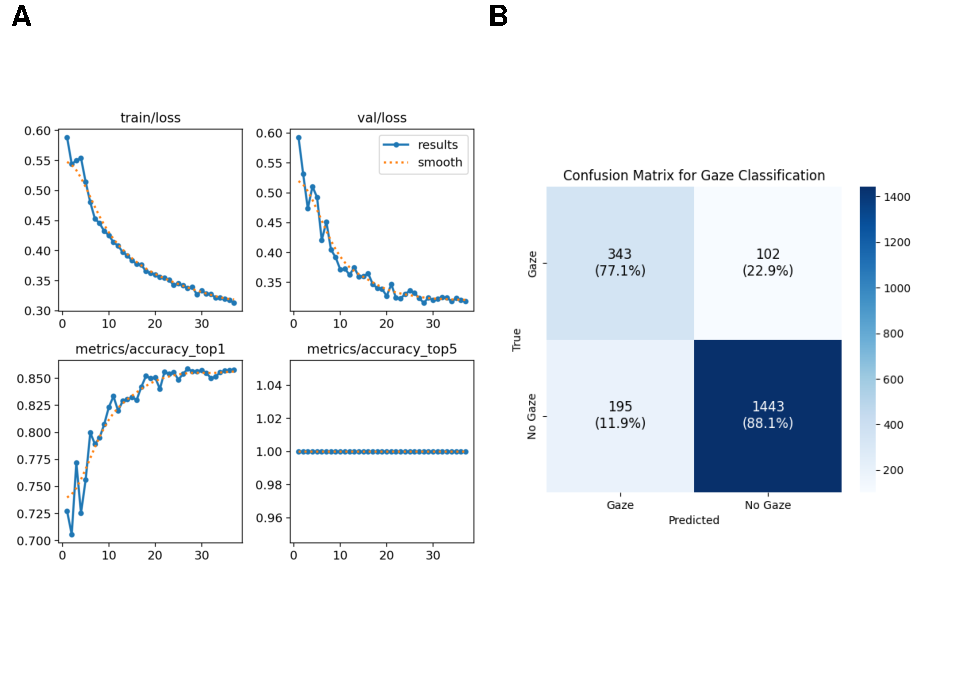
\includegraphics{Quantex_interaction_paper_files/figure-latex/gaze-loss-confusion-matrix-1} 

}

\caption{\textbf{A} - Training and Validation Loss Curves for the YOLO11x gaze classification model. \textbf{B} - Confusion Matrix for the YOLO11x gaze classification model trained on the Quantex dataset.}\label{fig:gaze-loss-confusion-matrix}
\end{figure}

Figure \ref{fig:gaze-loss-confusion-matrix} shows the cross-entropy loss curves for both training and validation. The steady decline in loss over time indicates that the model effectively learned to classify whether a person is looking in the direction of the child or not. The convergence of the training and validation loss curves suggests that the model generalizes well, as there is no indication of overfitting. Since gaze classification is a binary task, we used top-1 accuracy as the primary evaluation metric. Figure \ref{fig:gaze-loss-confusion-matrix}A also illustrates the increasing accuracy over time, confirming that the model progressively improves its ability to classify gaze correctly.

\subsubsection{Model Evaluation Metrics}\label{model-evaluation-metrics-1}

The YOLO11x gaze classification model achieved a precision of 0.64, a recall of 0.77, and an F1-score of 0.70 on the testing set. These metrics, summarized in table \ref{tab:gaze-metrics}, indicate that the model effectively distinguishes between gaze and no-gaze frames, though there is still room for improvement. The egocentric perspective of the dataset presents challenges, as faces are often partially occluded or blurred, making gaze classification difficult---even for human annotators, who occasionally required a second inspection to determine gaze direction.

\begin{table}[tbp]

\begin{center}
\begin{threeparttable}

\caption{\label{tab:gaze-metrics}Evaluation metrics for the YOLO11x gaze classification model trained on the Quantex dataset to classify whether a person is looking into the direction of the child wearing the camera or not. Precision, recall, and F1-score are given for the testing set.}

\begin{tabular}{lll}
\toprule
Precision & \multicolumn{1}{c}{Recall} & \multicolumn{1}{c}{F1-Score}\\
\midrule
0.64 & 0.77 & 0.70\\
\bottomrule
\end{tabular}

\end{threeparttable}
\end{center}

\end{table}

One of the primary challenges arises from cut-off faces, where the eyes are not always visible. In such cases, the model must rely on other facial features, such as head orientation or mouth position, to infer gaze direction. While this approach is often effective, it occasionally leads to misclassifications. Despite these difficulties, the model achieved a satisfactory recall, correctly identifying 77\% of all gaze frames.

More advanced gaze estimation methods---such as incorporating temporal information or leveraging additional facial landmarks---could further improve performance. However, given the constraints of our dataset and the focus on binary gaze classification, the YOLO11x model serves as a strong foundation for analyzing the gaze aspect of social interactions in egocentric video data.

\subsection{Proximity Heuristic}\label{sup-proximity}

Proximity between individuals is an important aspect of social interaction. Previous studies have shown that interpersonal distance can provide insights into the nature of relationships and social engagement (Hernández-Heredia et al., 2024; Janssen et al., 2024; Onnela et al., 2014). Since our dataset does not contain explicit proximity labels, we developed a heuristic approach to estimate the distance between the child and other individuals.

\subsubsection{Formula for Proximity Estimation}\label{formula-for-proximity-estimation-1}

We infer proximity from the size of the bounding boxes of detected faces, assuming that the size of these bounding boxes provides an implicit cue for proximity. Specifically, we infer that larger bounding boxes correspond to individuals closer to the camera, whereas smaller bounding boxes indicate individuals further away. The proximity value is calculated using the face area, defined as the product of the bounding box width and height. This computed size is then compared to predefined reference face sizes: one corresponding to a face very close to the camera (within arm's reach) and another representing a face further away (e.g., in the background or outdoors).

Due to the nonlinear relationship between face size and distance, where face area decreases quadratically as distance increases, a simple linear mapping would make small differences appear too large for close faces and too small for distant ones. To address this, we apply a logarithmic scaling approach, which maps the calculated face area to a proximity score between 0 and 1:

\[
\text{Proximity} = \frac{\ln(\text{Face Area}) - \ln(\text{Max Reference Area})}{\ln(\text{Min Reference Area}) - \ln(\text{Max Reference Area})}
\]

Where:

\begin{itemize}
\tightlist
\item
  \(\textbf{Face Area}\) is the area of the detected face, calculated as the width times the height of the bounding box.
\item
  \(\textbf{Max Reference Area}\) is the reference area corresponding to the furthest detectable face.
\item
  \(\textbf{Min Reference Area}\) is the reference area corresponding to the closest detectable face.
\end{itemize}

This logarithmic transformation ensures that proximity values are compressed for large faces (close to the camera) and stretched for small faces (farther away), making them perceptually meaningful. Since human sensitivity to size changes depends on relative differences rather than absolute ones, logarithmic scaling aligns with psychophysical principles of distance perception (Stevens \& Marks, 2017).

\begin{figure}

{\centering \includegraphics{Quantex_interaction_paper_files/figure-latex/proximity-heuristic-1} 

}

\caption{Proximity Heuristic examples. Example \textbf{A} shows a face far away from the camera (proximity score = 0.07), example \textbf{B} depicts a face slighlty closer (proximity score = 0.2). Example \textbf{C} shows a face quite close to the camera (proximity score = 0.6), and example \textbf{D} illustrates a face extremely close to the camera (proximity score = 1).}\label{fig:proximity-heuristic}
\end{figure}

\subsubsection{Incorporating Width-to-Height Ratio}\label{incorporating-width-to-height-ratio-1}

Along with face size, we use the width-to-height ratio of the detected face as a proximity cue. Reference aspect ratios for adults and children are based on front-facing images. If a detected face's aspect ratio deviates significantly from the expected ratio, we infer that the face is extremely close to the camera, causing partial cropping of the bounding box.

If the deviation exceeds a set threshold (\(\epsilon\)), the proximity score is set to 1:

\[
r_{\text{expected}} = \frac{w_{\text{expected}}}{h_{\text{expected}}}
\]

\[
\text{If} \quad |r_{\text{detected}} - r_{\text{expected}}| > \epsilon, \quad P = 1
\]

With (\(\epsilon\)=1), this heuristic efficiently estimates proximity using only image-based cues, avoiding the need for additional sensors. It helps analyze social interactions in egocentric recordings, offering insights into children's spatial relationships. Figure \ref{fig:proximity-heuristic} illustrates proximity scores from 0 (far) to 1 (very close).

\subsubsection{Proximity Heuristic Evaluation}\label{proximity-heuristic-evaluation}

To validate our proximity heuristic, we conducted a quality check using human annotations. A total of 364 frames (185 adult faces and 179 child faces) were evaluated by two independent annotators. Each annotator directly assigned a proximity value between 0 and 1, with 0 representing the furthest distance and 1 the closest.

Prior to the assessment task, annotators were shown the same reference images used for calculating the reference face sizes in the proximity estimation. They were informed that the closest reference image corresponded to a value of 1, while the furthest reference image corresponded to a value of 0. This ensured a shared understanding of the proximity scale and minimized subjective interpretation differences.

\begin{table}
\centering
\caption{\label{tab:proximity-metrics}Proximity evaluation metrics. The table shows the Pearson correlation coefficient (Pearson), Mean Absolute Error (MAE), Root Mean Squared Error (RMSE), Coefficient of Determination (R²), and Bias for the proximity heuristic compared to human annotations.}
\centering
\resizebox{\ifdim\width>\linewidth\linewidth\else\width\fi}{!}{
\begin{tabular}[t]{llllllllll}
\toprule
\multicolumn{1}{c}{ } & \multicolumn{3}{c}{all faces} & \multicolumn{3}{c}{adult faces} & \multicolumn{3}{c}{child faces} \\
\cmidrule(l{3pt}r{3pt}){2-4} \cmidrule(l{3pt}r{3pt}){5-7} \cmidrule(l{3pt}r{3pt}){8-10}
Metrics & \( prox_{mean} \) & \( prox_1 \) & \( prox_2 \) & \( prox_{mean} \) & \( prox_1 \) & \( prox_2\) & \( prox_{mean} \) & \( prox_1 \) & \( prox_2 \)\\
\midrule
Pearson & \textbf{0.9492} & 0.9373 & 0.9035 & \textbf{0.9548} & 0.9518 & 0.9078 & \textbf{0.9372} & 0.9163 & 0.8877\\
MAE & 0.0914 & 0.0947 & 0.1596 & 0.1015 & 0.0864 & 0.1573 & 0.0809 & 0.1033 & 0.1621\\
RMSE & 0.1111 & 0.1180 & 0.1875 & 0.1207 & 0.1086 & 0.1857 & 0.1001 & 0.1270 & 0.1893\\
R2 & 0.8403 & 0.8615 & 0.4588 & 0.8207 & 0.8861 & 0.4992 & 0.8381 & 0.7958 & 0.3518\\
Bias & 0.0682 & -0.0134 & 0.1498 & 0.0860 & 0.0254 & 0.1464 & 0.0499 & -0.0536 & 0.1533\\
\bottomrule
\end{tabular}}
\end{table}

\begin{figure}

{\centering 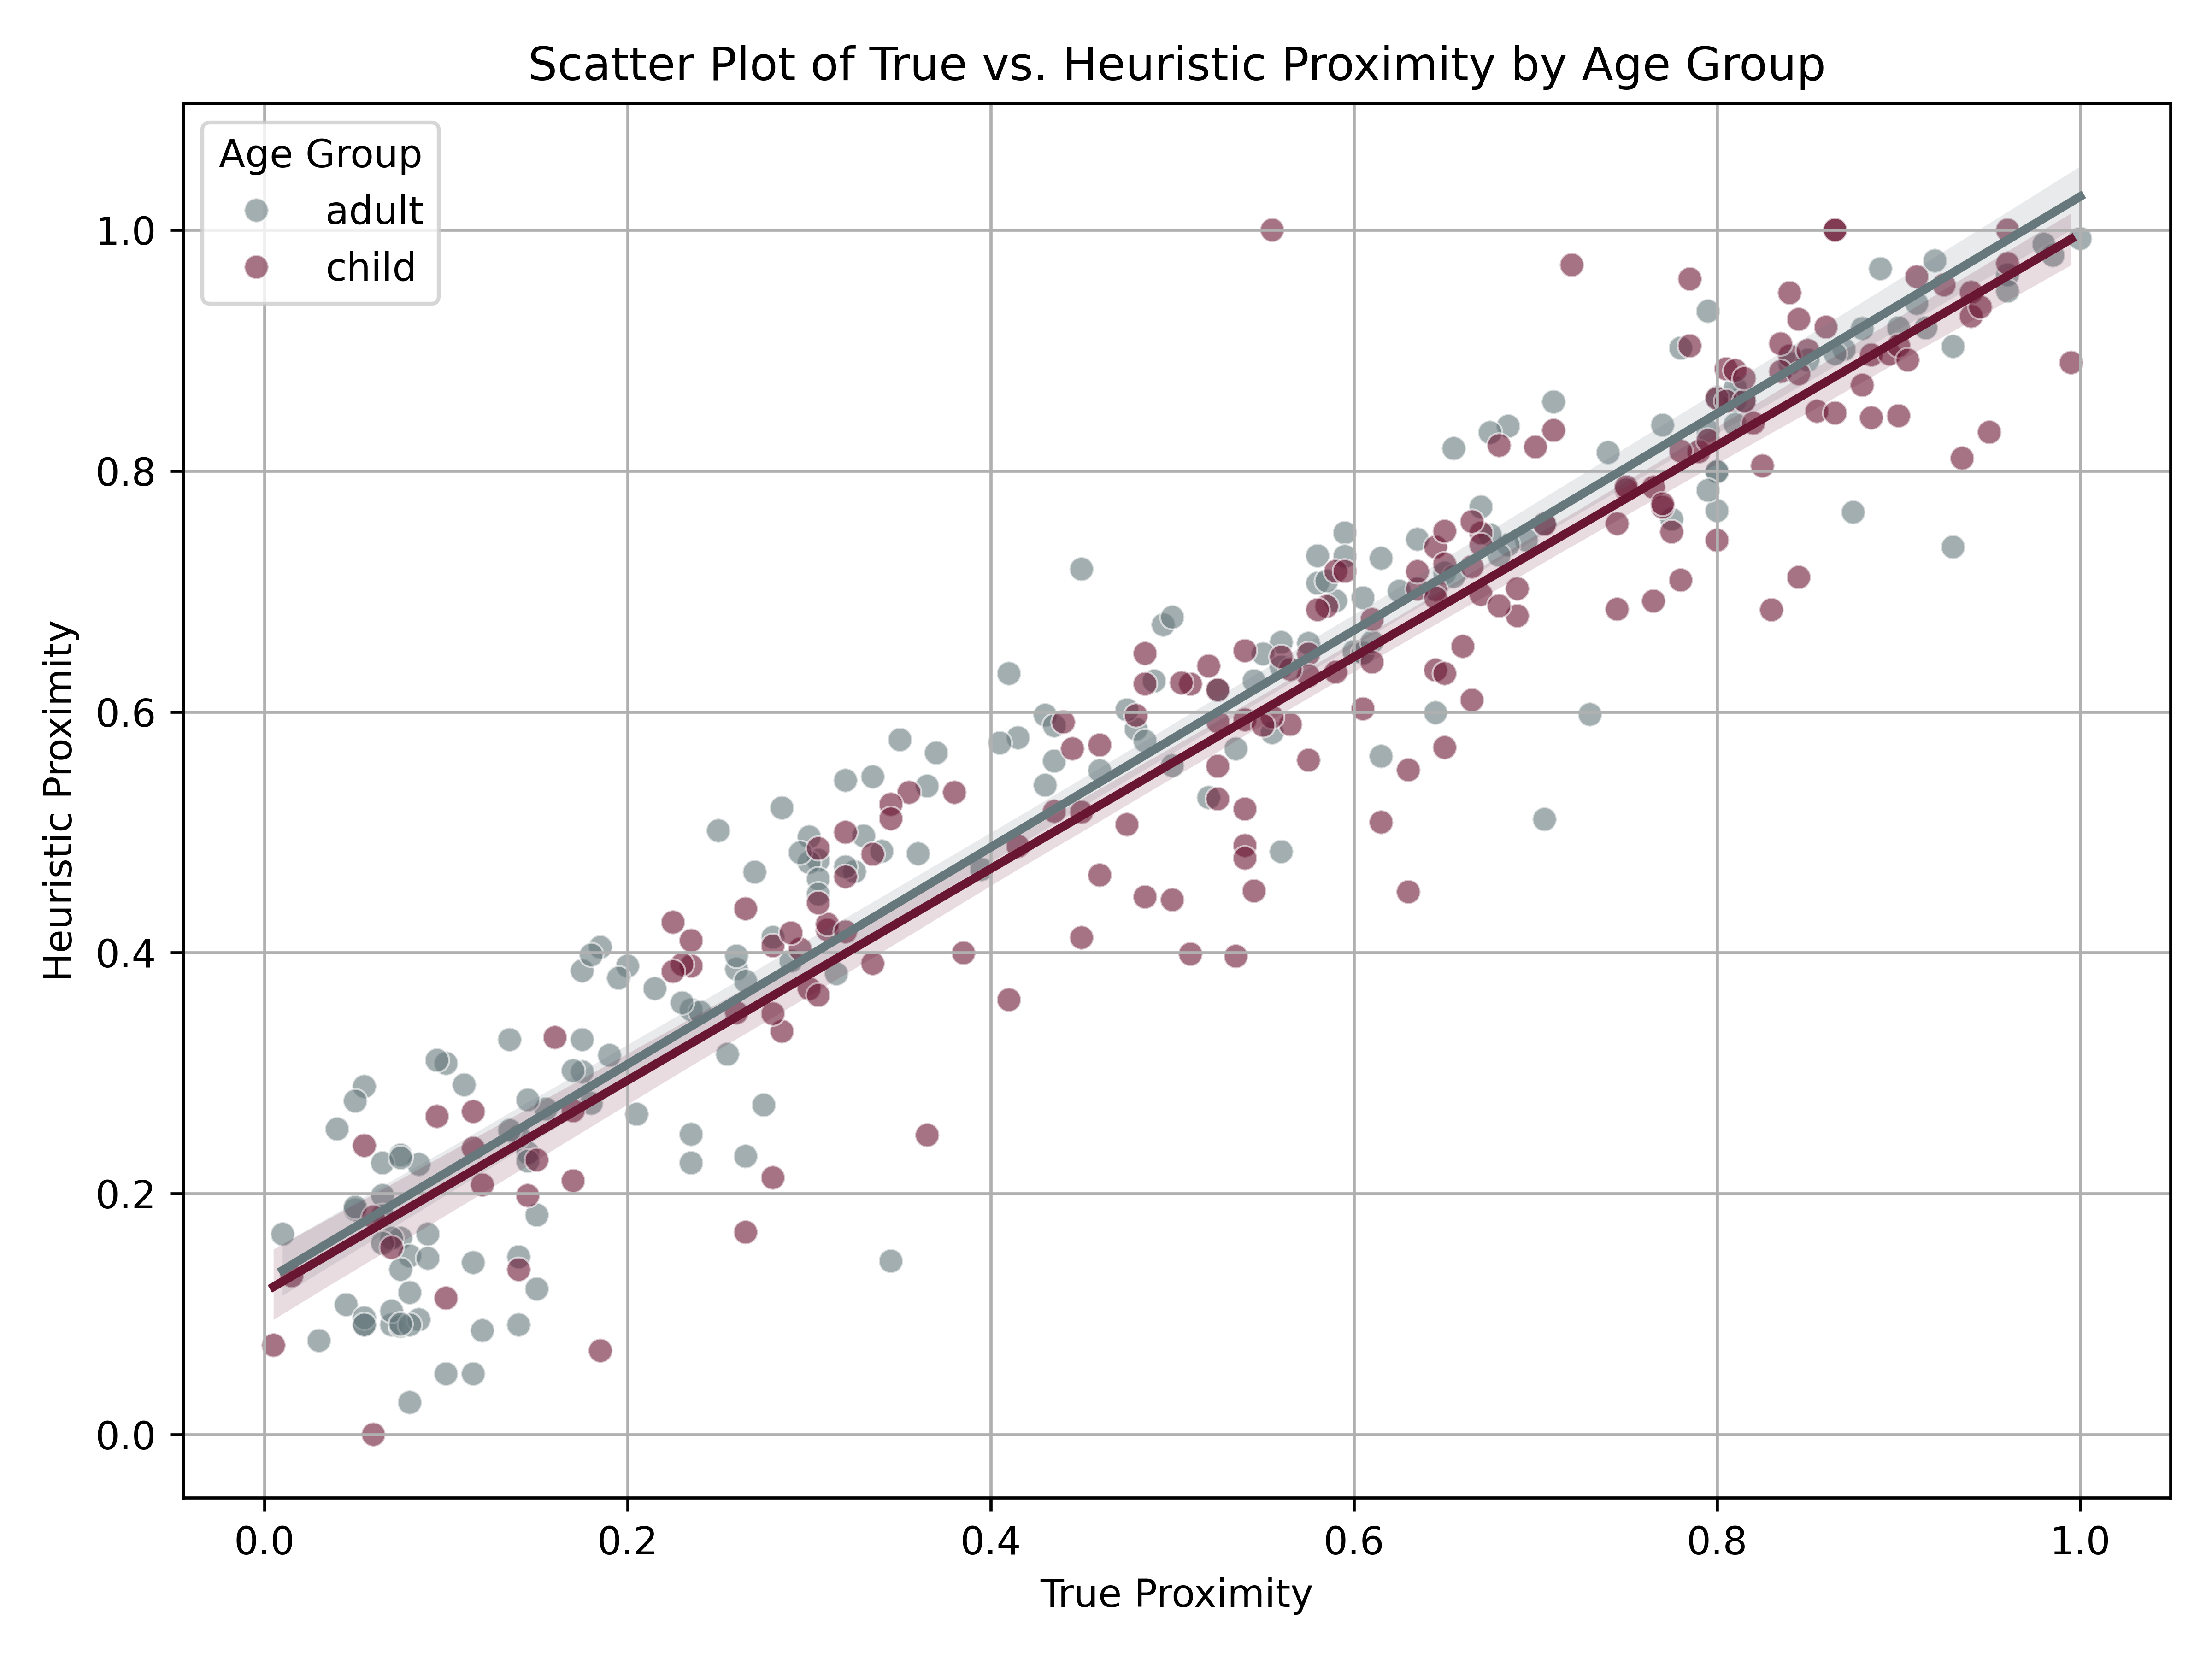
\includegraphics[width=450px]{images/proximity_eval_plot} 

}

\caption{The plot shows the correlation between the heuristic proximity values and the human-annotated proximity values for both adult and child faces. The red line represents the linear regression fit, while the shaded area indicates the 95\% confidence interval.}\label{fig:proximity-plot}
\end{figure}

Using this approach, the ground truth proximity for each frame is calculated as the mean of the two annotator ratings. We then compute how well the heuristic captures the human-annotated proximity values for both adult and child faces. Figure \ref{fig:proximity-plot} displays the correlation between the heuristic proximity values and the human-annotated proximity values for both adult and child faces. Both regression lines are close to the diagonal, indicating a strong correlation between the heuristic and human-annotated proximity values. Overall, the heuristic performs well, with a strong Pearson correlation coefficient of 0.95 for all faces, 0.95 for adult faces and 0.94 for child faces. The mean absolute error (MAE=0.09) for all faces is acceptably low and the coefficient of determination (R²=0.84) for all faces indicates that the heuristic explains a significant portion of the variance in human-annotated proximity values.
To conclude, the proximity heuristic provides a reliable estimate of interpersonal distance in our dataset, allowing us to add another reliable aspect of social interactions without the need for additional sensors or annotations.

\subsection{Participation Role Classifier}\label{sup-voice-direction}

Regarding the audio component of our interaction analysis, we aimed to classify speech not only by its presence but by its source and intended target. Specifically, we distinguish between four speech types: First, speech from the key child wearing the camera (KCHI), second, speech directed at the child from adults or other children (CDS), third, overheard speech (OHS), defined as conversations the child can hear but is not direcetly part of and fourth, general speech (SPEECH), which simply captures any type of speech. This distinction is crucial for understanding the interaction dynamics and the key child's role in the social context.

To achieve this, we adapted the Voice Type Classifier (VTC) (Lavechin et al., 2020), an open-source model originally trained to identify five voice types---key child, other child, female adult, male adult, and general speech. We restructured the model for our new four-class task and refer to this adapted version as the Participation Role Classifier (PRC).

Compared to the original VTC, the PRC enhanced model capacity and sequence modeling depth: the first-layer SincNet output channels were increased from 256 to 512, the bi-directional LSTM was replaced with a bi-directional GRU (3 layers, 512 hidden units), and the fully connected stack was deepened to 256--256--128 units. We also extended the input segment duration from 2.0 to 4.0 seconds to better capture turn-taking dynamics and adjusted the batch size accordingly. These changes improved the model's ability to distinguish overlapping and context-dependent speech events relevant to our classification task.

\begin{table}[tbp]

\begin{center}
\begin{threeparttable}

\caption{\label{tab:vtc-results}Performance of the Participation Role Classifier (PRC) on the ChildLens dataset. The table shows the F1 scores for each voice type (KCHI, CDS, OHS, SPEECH) and the average F1 score across all classes.}

\begin{tabular}{llllll}
\toprule
Dataset & \multicolumn{1}{c}{KCHI} & \multicolumn{1}{c}{CDS} & \multicolumn{1}{c}{OHS} & \multicolumn{1}{c}{SPEECH} & \multicolumn{1}{c}{AVG}\\
\midrule
ChildLens & 72.3 & 65.3 & 48.7 & cc & 44.6\\
\bottomrule
\end{tabular}

\end{threeparttable}
\end{center}

\end{table}

Although the Quantex dataset lacks explicit audio labels, we validated the adapted model architecture on ChildLens, a similarly structured, labeled dataset from our lab (REFERENCE TO CHILDLENS PAPER). The PRC achieved an average F1 score of 65.40 on ChildLens, (Table \ref{tab:vtc-results}) comparable to the original VTC's F1 score (57.30) on its benchmark dataset (Lavechin et al., 2020). These results support the architecture's robustness and suitability for our analysis.

\subsection{Results and Analysis}\label{sup-results}

\newpage

\section{References}\label{references-1}

\begingroup
\setlength{\parindent}{-0.5in}
\setlength{\leftskip}{0.5in}

\phantomsection\label{refs}
\begin{CSLReferences}{1}{0}
\bibitem[\citeproctext]{ref-carpendaleWhatMakesUs2020}
Carpendale, J., \& Lewis, C. (2020). \emph{What {Makes Us Human}: {How Minds Develop} through {Social Interactions}} (1st ed.). Routledge. \url{https://doi.org/10.4324/9781003125105}

\bibitem[\citeproctext]{ref-chengAppearancebasedGazeEstimation2021}
Cheng, Y., Wang, H., Bao, Y., \& Lu, F. (2021). Appearance-based {Gaze Estimation With Deep Learning}: {A Review} and {Benchmark}. \url{https://doi.org/10.48550/ARXIV.2104.12668}

\bibitem[\citeproctext]{ref-daiLongitudinalDataCollection2022}
Dai, S., Bouchet, H., Karsai, M., Chevrot, J.-P., Fleury, E., \& Nardy, A. (2022). Longitudinal data collection to follow social network and language development dynamics at preschool. \emph{Scientific Data}, \emph{9}(1), 777. \url{https://doi.org/10.1038/s41597-022-01756-x}

\bibitem[\citeproctext]{ref-hernandez-herediaProximitySensorMeasuring2024}
Hernández-Heredia, T. K., Reyes-Manzano, C. F., Flores-Hernández, D. A., Ramos-Fernández, G., \& Guzmán-Vargas, L. (2024). Proximity {Sensor} for {Measuring Social Interaction} in a {School Environment}. \emph{Sensors}, \emph{24}(15), 4822. \url{https://doi.org/10.3390/s24154822}

\bibitem[\citeproctext]{ref-heyesCognitiveGadgetsCultural2018}
Heyes, C. M. (2018). \emph{Cognitive gadgets: The cultural evolution of thinking}. Cambridge (Mass.): Harvard University press.

\bibitem[\citeproctext]{ref-janssenTrackingRealtimeProximity2024}
Janssen, L. H. C., Verkuil, B., Nedderhoff, A., Van Houtum, L. A. E. M., Wever, M. C. M., \& Elzinga, B. M. (2024). Tracking real-time proximity in daily life: {A} new tool to examine social interactions. \emph{Behavior Research Methods}, \emph{56}(7), 7482--7497. \url{https://doi.org/10.3758/s13428-024-02432-1}

\bibitem[\citeproctext]{ref-jocherUltralyticsYOLO112024}
Jocher, G., \& Qiu, J. (2024). \emph{Ultralytics {YOLO11}}. Retrieved from \url{https://github.com/ultralytics/ultralytics}

\bibitem[\citeproctext]{ref-kellnhoferGaze360PhysicallyUnconstrained2019}
Kellnhofer, P., Recasens, A., Stent, S., Matusik, W., \& Torralba, A. (2019). Gaze360: {Physically Unconstrained Gaze Estimation} in the {Wild}. \url{https://doi.org/10.48550/ARXIV.1910.10088}

\bibitem[\citeproctext]{ref-khanamYOLOv11OverviewKey2024}
Khanam, R., \& Hussain, M. (2024, October 23). {YOLOv11}: {An Overview} of the {Key Architectural Enhancements}. \url{https://doi.org/10.48550/arXiv.2410.17725}

\bibitem[\citeproctext]{ref-lavechinOpensourceVoiceType2020}
Lavechin, M., Bousbib, R., Bredin, H., Dupoux, E., \& Cristia, A. (2020). An open-source voice type classifier for child-centered daylong recordings. \url{https://doi.org/10.48550/ARXIV.2005.12656}

\bibitem[\citeproctext]{ref-lemaignanPInSoRoDatasetSupporting2018}
Lemaignan, S., Edmunds, C. E. R., Senft, E., \& Belpaeme, T. (2018). The {PInSoRo} dataset: {Supporting} the data-driven study of child-child and child-robot social dynamics. \emph{PLOS ONE}, \emph{13}(10), e0205999. \url{https://doi.org/10.1371/journal.pone.0205999}

\bibitem[\citeproctext]{ref-liGeneralizedFocalLoss2020}
Li, X., Wang, W., Wu, L., Chen, S., Hu, X., Li, J., \ldots{} Yang, J. (2020, June 8). Generalized {Focal Loss}: {Learning Qualified} and {Distributed Bounding Boxes} for {Dense Object Detection}. \url{https://doi.org/10.48550/arXiv.2006.04388}

\bibitem[\citeproctext]{ref-linMicrosoftCOCOCommon2014}
Lin, T.-Y., Maire, M., Belongie, S., Bourdev, L., Girshick, R., Hays, J., \ldots{} Dollár, P. (2014). Microsoft {COCO}: {Common Objects} in {Context}. \url{https://doi.org/10.48550/ARXIV.1405.0312}

\bibitem[\citeproctext]{ref-loshchilovSGDRStochasticGradient2017}
Loshchilov, I., \& Hutter, F. (2017, May 3). {SGDR}: {Stochastic Gradient Descent} with {Warm Restarts}. \url{https://doi.org/10.48550/arXiv.1608.03983}

\bibitem[\citeproctext]{ref-onnelaUsingSociometersQuantify2014}
Onnela, J.-P., Waber, B. N., Pentland, A., Schnorf, S., \& Lazer, D. (2014). Using sociometers to quantify social interaction patterns. \emph{Scientific Reports}, \emph{4}(1), 5604. \url{https://doi.org/10.1038/srep05604}

\bibitem[\citeproctext]{ref-piagetPartCognitiveDevelopment1964}
Piaget, J. (1964). Part {I}: {Cognitive} development in children: {Piaget} development and learning. \emph{Journal of Research in Science Teaching}, \emph{2}(3), 176--186. \url{https://doi.org/10.1002/tea.3660020306}

\bibitem[\citeproctext]{ref-rogoffImportanceUnderstandingChildrens2018}
Rogoff, B., Dahl, A., \& Callanan, M. (2018). The importance of understanding children's lived experience. \emph{Developmental Review}, \emph{50}, 5--15. \url{https://doi.org/10.1016/j.dr.2018.05.006}

\bibitem[\citeproctext]{ref-rossanoHow24yearold2022}
Rossano, F., Terwilliger, J., Bangerter, A., Genty, E., Heesen, R., \& Zuberbühler, K. (2022). How 2- and 4-year-old children coordinate social interactions with peers. \emph{Philosophical Transactions of the Royal Society B: Biological Sciences}, \emph{377}(1859), 20210100. \url{https://doi.org/10.1098/rstb.2021.0100}

\bibitem[\citeproctext]{ref-shahDriverGazeEstimation2022}
Shah, S. M., Sun, Z., Zaman, K., Hussain, A., Shoaib, M., \& Pei, L. (2022). A {Driver Gaze Estimation Method Based} on {Deep Learning}. \emph{Sensors}, \emph{22}(10), 3959. \url{https://doi.org/10.3390/s22103959}

\bibitem[\citeproctext]{ref-smithDevelopingInfantCreates2018}
Smith, L. B., Jayaraman, S., Clerkin, E., \& Yu, C. (2018). The {Developing Infant Creates} a {Curriculum} for {Statistical Learning}. \emph{Trends in Cognitive Sciences}, \emph{22}(4), 325--336. \url{https://doi.org/10.1016/j.tics.2018.02.004}

\bibitem[\citeproctext]{ref-stevensPsychophysicsIntroductionIts2017}
Stevens, S. S., \& Marks, L. E. (2017). \emph{Psychophysics: {Introduction} to {Its Perceptual}, {Neural}, and {Social Prospects}} (1st ed.). Routledge. \url{https://doi.org/10.4324/9781315127675}

\bibitem[\citeproctext]{ref-tervenLossFunctionsMetrics2024}
Terven, J., Cordova-Esparza, D. M., Ramirez-Pedraza, A., Chavez-Urbiola, E. A., \& Romero-Gonzalez, J. A. (2024, October 12). Loss {Functions} and {Metrics} in {Deep Learning}. \url{https://doi.org/10.48550/arXiv.2307.02694}

\bibitem[\citeproctext]{ref-tomaselloCulturalOriginsHuman2009}
Tomasello, M. (2009). \emph{Cultural {Origins} of {Human Cognition}}. Cambridge: Harvard University Press.

\bibitem[\citeproctext]{ref-vygotskyMindSocietyDevelopment1978}
Vygotsky, L. S. (1978). \emph{Mind in {Society}: {The Development} of {Higher Psychological Processes}}. Cambridge, MA: Harvard University Press.

\bibitem[\citeproctext]{ref-zhangETHXGazeLargeScale2020}
Zhang, X., Park, S., Beeler, T., Bradley, D., Tang, S., \& Hilliges, O. (2020). {ETH-XGaze}: {A Large Scale Dataset} for {Gaze Estimation} under {Extreme Head Pose} and {Gaze Variation}. \url{https://doi.org/10.48550/ARXIV.2007.15837}

\bibitem[\citeproctext]{ref-zhangAppearancebasedGazeEstimation2015}
Zhang, X., Sugano, Y., Fritz, M., \& Bulling, A. (2015). Appearance-based gaze estimation in the wild. \emph{2015 {IEEE Conference} on {Computer Vision} and {Pattern Recognition} ({CVPR})}, 4511--4520. Boston, MA, USA: IEEE. \url{https://doi.org/10.1109/CVPR.2015.7299081}

\bibitem[\citeproctext]{ref-zhangItsWrittenAll2016}
Zhang, X., Sugano, Y., Fritz, M., \& Bulling, A. (2016). \emph{It's {Written All Over Your Face}: {Full-Face Appearance-Based Gaze Estimation}}. \url{https://doi.org/10.48550/ARXIV.1611.08860}

\bibitem[\citeproctext]{ref-zhangMPIIGazeRealWorldDataset2019}
Zhang, X., Sugano, Y., Fritz, M., \& Bulling, A. (2019). {MPIIGaze}: {Real-World Dataset} and {Deep Appearance-Based Gaze Estimation}. \emph{IEEE Transactions on Pattern Analysis and Machine Intelligence}, \emph{41}(1), 162--175. \url{https://doi.org/10.1109/TPAMI.2017.2778103}

\end{CSLReferences}

\endgroup

\newpage

\section{Appendix}\label{appendix}


\end{document}
